\RequirePackage{fix-cm}
\documentclass[smallextended]{svjour3}      
\smartqed  % flush right qed marks, e.g. at end of proof
\usepackage{graphicx}
\usepackage{mathptmx} 
\journalname{Preprint}
%%%%  Our packages 
\usepackage{color}
\usepackage{algorithmic,algorithm}
%%\usepackage[]{algorithm2e}
\renewcommand{\algorithmiccomment}[1]{\hfill$\rhd???$\textit{#1}}
\usepackage{mathtools}
%%\usepackage{scalerel}#
\usepackage{amsfonts}
\usepackage{amssymb}
\usepackage{natbib}
\bibliographystyle{mde}
\setcitestyle{authoryear,open={(},close={)}}
\let\cite\citep



%\usepackage{natbib}
%\bibliographystyle{agsm}
%\setcitestyle{authoryear,open={(},close={)}}
%%\definecolor{violet}{RGB}{127,0,255}




%%%% Abbreviations  
\newcommand{\rev}[1]{\begingroup\color{blue}#1\endgroup}
\newcommand{\TODO}[1]{\begingroup\color{red}#1\endgroup}
\newcommand{\remove}[1]{\begingroup\tiny\color{yellow}#1\endgroup}
%\newcommand{\PFS}[1]{\begingroup\color{blue}#1\endgroup}
%%\newcommand{\PFSNEW}[1]{\begingroup\color{violet}#1\endgroup}

\newcommand{\mh}[1]{\begingroup\color{magenta}#1\endgroup}
%\newcommand{\mhcomment}[1]{\begingroup\emph{\color{red}#1}\endgroup}
%\newcommand{\yangjing}[1]{\begingroup\color{green}#1\endgroup}
%\newcommand{\TRY}[1]{\begingroup\color{violet}#1\endgroup}


\newcommand{\Ro}{\mathrel{\overset{0}{\sim}}}
\newcommand{\Rl}{\mathrel{\overset{1}{\sim}}}
\newcommand{\Rlstar}{\mathrel{\overset{1\star}{\sim}}}
\newcommand{\Rldstar}{\mathrel{\overset{1\star}{\rightharpoonup}}}

\newcommand{\Rk}{\mathrel{\overset{\ge k}{\sim}}}
\newcommand{\Rld}{\mathrel{\overset{1}{\rightharpoonup}}}
\newcommand{\Rldk}{\mathrel{\overset{k}{\rightharpoonup}}}
\newcommand{\Rd}{\mathrel{\rightsquigarrow}}
\renewcommand{\P}{\mathbb{P}}
\newcommand{\lca}[1]{\mathop{lca}(#1)}
\newcommand{\rt}[1]{\ensuremath{\mathsf{#1}}}

\newcommand{\Mo}{\ensuremath{M^\odot}}
\renewcommand{\varnothing}{\odot}


%\newcommand{\overlap}{\between}

\newtheorem{thm}{Theorem}
%\newtheorem{lemma}[thm]{Lemma}
\newtheorem{cor}[thm]{Corollary}
\newtheorem{prop}[thm]{Proposition}

\begin{document}
\setlength{\itemindent}{1cm}



\title{Inferring Phylogenetic Trees from the Knowledge of Rare Evolutionary
  Events}

\author{Marc Hellmuth  \and Maribel Hernandez-Rosales \and Yangjing Long \and 
Peter F.\ Stadler }

\institute{Marc Hellmuth \at
        Department of Mathematics and Computer Science, 
        University of Greifswald, 
        Walther-Rathenau-Stra{\ss}e 47, D-17487 Greifswald, Germany, and
        Center for Bioinformatics, Saarland University, Building E 2.1, 
        P.O.\ Box 151150,
        D-66041 Saarbr{\"u}cken, Germany\\
        \email{mhellmuth@mailbox.org}
        \and
        Maribel Hernandez-Rosales \at
        CONACYT-Instituto de Matem{\'a}ticas, UNAM Juriquilla,
        Blvd. Juriquilla 3001,
        76230 Juriquilla, Quer{\'e}taro, QRO, M{\'e}xico\\
        \email{maribel@im.unam.mx}
        \and
        Yangjing Long \at
        School of Mathematical Sciences,
        Shanghai Jiao Tong university, Dongchuan Road 800, 200240 Shanghai, 
        China\\
        \email{yjlong@sjtu.edu.cn}
        \and
        Peter F.\ Stadler \at
        Bioinformatics Group, Department of Computer Science; and
        Interdisciplinary Center of Bioinformatics, University of Leipzig,
        H{\"a}rtelstra{\ss}e 16-18, D-04107 Leipzig, and 
        Max-Planck-Institute for Mathematics in the Sciences,
        Inselstra{\ss}e 22, D-04103 Leipzig, and 
        Inst.\ f.\ Theoretical Chemistry, University of Vienna,
        W{\"a}hringerstra{\ss}e 17, A-1090 Wien, Austria, and 
        Santa Fe Institute, 1399 Hyde Park Rd., Santa Fe,
        NM 87501, USA \\
        \email{studla@bioinf.uni-leipzig.de}
}

\maketitle

\begin{abstract} 
  Rare events have played an increasing role in molecular phylogenetics as
  potentially homoplasy-poor characters. In this contribution we analyze
  the phylogenetic information content from a combinatorial point of view
  by considering the binary relation on the set of taxa defined by the
  existence of single event separating two taxa. We show that the
  graph-representation of this relation must be a tree.  Moreover, we
  characterize completely the relationship between the tree of such
  relations and the underlying phylogenetic tree. With directed operations
  such as tandem-duplication-random-loss events in mind we demonstrate how
  non-symmetric information constrains the position of the root in the
  partially reconstructed phylogeny.

  \keywords{Phylogenetic Combinatorics \and Rare events \and Binary
    relations}
\end{abstract} 

\sloppy

\section{Introduction}

Shared derived characters (synapomorphies or ``Hennigian markers'') that
are unique to specific clades form the basis of classical cladistics
\cite{Hennig:50}. In the context of molecular phylogenetics \emph{rare
  genomic changes (RGCs)} can play the same important role
\cite{Rokas:00,Boore:06}. RGCs corresponds to rare mutational events that
are very unlikely to occur multiple times and thus are (almost) free of
homoplasy. A wide variety of processes and associated markers have been
proposed and investigated. Well-studied RGCs include presence/absence
patterns of protein-coding genes \cite{Dutilh:08} as well as microRNAs
\cite{Sempere:06}, retroposon integrations \cite{Shedlock:00}, insertions
and deletions (indels) of introns \cite{Rogozin:05}, pairs of mutually
exclusive introns (NIPs) \cite{Krauss:08a}, protein domains
\cite{Deeds:05,Yang:05}, RNA secondary structures \cite{Misof:03}, protein
fusions \cite{Stechmann:03}, changes in gene order
\cite{Sankoff:82,Boore:98,Lavrov:07}, metabolic networks
\cite{Forst:01,Forst:06a,Mazurie:08}, transcription factor binding sites
\cite{Prohaska:04a}, insertions and deletions of arbitrary sequences
\cite{Simmons:00,Ashkenazy:14,Donath:14a}, and variations of the genetic
code \cite{Abascal:12}. RGCs clearly have proved to be phylogenetically
informative and helped to resolve many of the phylogenetic questions where
sequence data lead to conflicting or equivocal results.

Not all RGCs behave like cladistic characters, however. While
presence/absence characters are naturally stored in character matrices
whose columns can vary independently, this is not the case e.g.\ for gene
order characters. From a mathematical point of view, character-based
parsimony analysis requires that the mutations have a product structure in
which characters are identified with factors and character states can vary
independently of each other \cite{Wagner:03a}. This assumption is violated
whenever changes in the states of two distinct characters do not commute.
Gene order is of course the prime example on non-commutative events.
  
Three strategies have been pursued in such cases. Most importantly, the
analog of the parsimony approach is considered for a particular
non-commutative model. For the genome rearrangements an elaborate theory has
been developed that considers various types of operations on (usually
signed) permutations. Already the computation of editing distances is
non-trivial. An added difficulty is that the interplay of different
operations such as reversals, transpositions, and
tandem-duplication-random-loss (TDRL) events is difficult to handle
\cite{Bernt:07a,Hartmann:16}. An alternative is to focus on distance-based
methods \cite{Wang:06}. Since good rate models are usually unavailable,
distance measures usually are not additive and thus fail to precisely
satisfy the assumptions underlying the most widely used methods such as
neighbor joining. The third strategy is to convert the non-commutative data
structure into a presence-absence structure, e.g., by using pairwise
adjacencies \cite{Tang:05} as representation of permutations or using list
alignments in which rearrangements appear as pairs of insertions and
deletions \cite{Fritzsch:06a}. While this yields character matrices that
can be fed into parsimony algorithms, these can only result in approximate
heuristics.

While it tends to be difficult to disentangle multiple, super-imposed
complex changes such as genome rearrangements or tandem duplication, it is
considerably simpler to recognize whether two genes or genomes differ by a
single RGC operation. It make sense therefore to ask just how much
phylogenetic information can be extracted from elementary RGC events. Of
course, we cannot expect that a single RGC will allow us to (re)construct a
detailed phylogeny. It can, however, provide us with solid, well-founded
constraints. Furthermore, we can hope that the combination of such
constraints can be utilized as a practicable method for phylogenetic
inference. Recently we have shown that orthology assignments in large gene
families imply triples that must be displayed by the underlying species
tree \cite{HernandezRosales:12a,Hellmuth:13a} \TODO{also cite Marbrouk
  stuff here?}. In a phylogenomics setting a sufficient number of such
triple constraints can be collected to yield fully resolved phylogenetic
trees \cite{Hellmuth:15a}, see \citet{HW:16b} for an overview.

A plausible application scenario for our setting is the rearrangement of
mitogenomes \cite{Sankoff:82}. Since mitogenomes are readily and cheaply
available, the taxon sampling is sufficiently dense so that the gene orders
often differ by only a single rearrangement or not at all. These cases are
identifiable with near certainty \cite{Bernt:07a}. Moreover, some RGC are
inherently directional. Probably the best known example is the tandem
duplication random loss (TDRL) operation \cite{Chaudhuri:06}. We will
therefore also consider a directed variant of the problem.

In this contribution, we ask how much phylogenetic information can be
retrieved from single RGCs. More precisely, we consider a scenario in which
we can, for every pair of taxa distinguish, for a given type of RGC,
whether $x$ and $y$ have the same genomic state, whether $x$ and $y$ differ
by exactly one elementary change, or whether their distance is larger than
a single operation. We formalize this problem in the following way. Given a
relation $\sim$ is there a phylogenetic tree $T$ with an edge labeling
$\lambda$ (marking the elementary events) such that $x\sim y$ if and only
if edge labeling along the unique path $\mathbb{P}(x,y)$ for $x$ to $y$ in
$T$ has a certain prescribed property $\Pi$. After defining the necessary
notation and preliminaries, we give a more formal definition of the general
problem in section~\ref{sect:theory}.

\rev{The graphs defined by path relations on a tree are closely related to
  \emph{pairwise compatibility graphs} (PCGs). A graph $G =(V,E)$ is a PCG
  if there is a tree $T$ with leaf set $V$, a positive edge-weight function
  $w:E(T)\to \mathbb{R}^+$, and two nonnegative real numbers $d_{\min}\le
  d_{\max}$ such that there is an edge $uv \in E(G)$ if and only if
  $d_{\min}\leq d_{T,w}(x,y) \leq d_{\max}$, where $d_{T,w}(x,y)$ is the
  sum of the weights of the edges on the unique path $\mathbb{P}(x,y)$ in
  $T$. One writes $G = \mathrm{PCG}(T, w, d_{\min} , d_{\max})$.} In this
contribution we will primarily be interested in the special case where
$\Pi$ is ``a single event along the path''. \rev{Although PCGs have been
  studied extensively, see e.g.,
  \citet{PCGsurvey,YHTR:08,YBR:10,CMPS:13,MR:13,DMR:13}, the questions are
  different from our motivation and, to out knowledge, there no results
  have been obtained that would simplify the characterization of the PGCs
  corresponding to the ``single-1-relation'' in Section~\ref{sect:single1}.
  PCGs, furthermore are always treated as undirected graphs in the
  literature.  We also consider a antisymmetric (Section~\ref{sect:1dir})
  and a general directed (Section~\ref{sect:mixed}) version of the
  single-1-relation motivated by RGCs with directional information.}

\rev{The main result of the contribution can be summarized as follows: (i)
  The graph of a single-1-relation is always a forrest. (ii) If the
  single-1-relation is connected, there is a unique minimally resolved tree
  that explain the relation. The same holds true for the connected
  components of an arbitrary relation. (iii) Analogous results hold for the
  anti-symmetric and the mixed variants of the single-1-relation. In this
  case not only the tree topology but also the position the of the root can
  be determined or at least constrained.}


\section{Preliminaries}
\label{sec:prelim}

\subsection{Basic Notation} 

We largely follow the notation and terminology of \rev{the book by}
\citet{sem-ste-03a}. Throughout, $X$ denotes always a finite set of at
least three taxa. We will consider both undirected and directed graphs
$G=(V,E)$ with finite vertex set $V(G)\coloneqq V$ and edge set or arc set
$E(G)\coloneqq E$.  For a digraph $G$ we write $\underline{G}$ for its
\emph{underlying (undirected) graph} where $V(G)=V(\underline{G})$ and
$\{x,y\}\in E(\underline{G})$ if $(x,y)\in E(G)$ or $(y,x)\in E(G)$. Thus,
$\underline{G}$ is obtained from $G$ by ignoring the direction of edges.
For simplicity, edges $\{x,y\}\in E(G)$ (in the undirected case) and arcs
$(x,y)\in E(G)$ (in the directed case) will be both denoted by $xy$.

The representation $G(R)=(V,E)$ of a relation $R\subseteq V\times V$ has
vertex set $V$ and edge set $E=\{xy\mid (x,y)\in R\}$. If $R$ is
irreflexive, then $G$ has no loops. If $R$ is symmetric, we regard $G(R)$
as an undirected graph. A \emph{clique} is a complete subgraph that is
maximal w.r.t.\ inclusion. An equivalence relation is \emph{discrete} if
all its equivalence classes consist of single vertices.

A tree $T=(V,E)$ is a connected cycle-free undirected graph.  The vertices
of degree $1$ in a tree are called leaves, all other vertices of $T$ are
called \emph{inner vertices}. 
An edge of $T$ is \emph{interior} if both of
its end vertices are interior vertices. 
\rev{For technical reasons, we call a vertex $v$ an inner vertex and leaf
if $T$ is a single vertex graph
$(\{v\},\emptyset)$. However, if 
$T$ is an edge $vw$ we refer to $v$ and $w$ as leaves but not
as inner vertices. Hence, in this case the edge $vw$ is not an
interior edge}


A \emph{star} $S_m$ with $m$ leaves
is a tree that has at most one inner vertex. A \emph{path} $P_n$ (on $n$
vertices) is a tree with two leaves and $n-3$ interior edges.  There is a
unique path $\mathbb{P}(x,y)$ connecting any two vertices $x$ and $y$ in a
tree $T$. We write $e\in\mathbb{P}(x,y)$ if the edge $e$ connects two
adjacent vertices along $\mathbb{P}(x,y)$.  We say that a directed graph is
a tree if its underlying undirected graph is a tree.  A directed path $P$
is a tree on vertices $x_1,\dots,x_n$ s.t. $x_ix_{i+1}\in E(P)$, $1\leq
i\leq n-1$. A graph is a forest if all its connected components are trees.

A tree is \emph{rooted} if there is a distinguished vertex $\rho\in V$
called the \emph{root}. Throughout this contribution we assume that the
root is an interior vertex. \rev{  Given a rooted tree $T=(V,E)$, there is a partial
order $\preceq$ on $V$ defined as  $ v \preceq u$ if 
$u$ lies on the path from $v$ to the root. Obviously,
the root is the unique maximal element w.r.t\ $\preceq$.
For a non-empty subset of $W\subseteq V$, we define $\lca{W}$, or
the \emph{least common ancestor of $W$}, to be the unique
$\preceq_T$-minimal vertex of $T$ that is an ancestor of every vertex in
$W$. In case $W=\{x,y \}$, we put $\lca{x,y}:=\lca{\{x,y\}}$.}
%%In rooted trees, the first inner vertex
%$\lca{x,y}$ that lies on both unique paths from two vertices $x$, resp.,
%$y$ to the root, is called \emph{lowest common ancestor} of $x$ and $y$.
If $T$ is rooted, then by definition $\lca{x,y}$ is a uniquely defined
inner vertex along $\mathbb{P}(x,y)$.

We write $L(v)$ for the set of leaves in the subtree below a fixed vertex
$v$, i.e., $L(v)$ is the set of all leaves for which $v$ is located on the
unique path from $x\in L(v)$ to the root of $T$. The \emph{children} of an
inner vertex $v$ are its direct descendants, i.e., vertices $w$ with $vw\in
E(T)$ s.t.\ that $w$ is further away from the root than $v$.  A rooted or
unrooted tree that has no vertices of degree two \rev{(except possibly the root of $T$)}
%(with the possible
%exception that $T$ is a single, distinguished root node) 
and leaf set $X$
is called a \emph{phylogenetic tree $T$ (on $X$)}.

Suppose $X'\subseteq X$. A phylogenetic tree $T$ on $X$ \emph{displays} a
phylogenetic tree $T'$ on $X'$ if $T'$ can be obtained from $T$ by a series
of vertex deletions, edge deletions, and suppression of vertices of degree
$2$ other than possibly the root, i.e., the replacement of an interior
vertex $u$ and its two incident edges $e'$ and $e''$ by a single edge $e$,
cf.\ \rev{Def.\ 6.1.2 in the book by \citet{sem-ste-03a}}. In the rooted
case, only a vertex between two \rev{incident} edges may be suppressed;
furthermore, if $X'$ is contained in a single subtree, then the $\lca{X'}$
becomes the root of $T'$. It is useful to note that $T'$ is displayed by
$T$ if and only if it can be obtained from $T$ step-wisely by removing an
arbitrarily selected leaf $y\in X\setminus X'$, its incident edge $e=yu$,
and suppression of $u$ provided $u$ has degree $2$ after removal of $e$.


\remove{ ******* START REMOVAL splits *********** \TODO{  -- should keeps the basics, that are needed 
for quartets - if quartets are used.}

A \emph{partial split} of X, or a \emph{partial X-split}, is a partition of
a subset of $X$ into two disjoint non-empty subsets $A$ and $B$, denoted by
$A|B$. Note, there is no difference between $A|B$ and $B|A$. If $A\cup
B=X$, then $A|B$ is called a \emph{(full) X-split}. For a split $A|B$ with
$A=\{a_1,\dots,a_i\}$ and $B=\{b_1,\dots,b_j\}$ we will write
$a_1,\dots,a_i|b_1,\dots,b_j$ instead of
$\{a_1,\dots,a_i\}|\{b_1,\dots,b_j\}$.  A partial X-split $A|B$ is
\emph{trivial} if $\min\{|A|, |B|\} = 1$.

Each edge $e\in E(T)$ of a tree $T$ gives rise to a split, that is, if one
removes $e$ from $T$ one obtains two distinct trees $T_1$ and $T_2$ with
leaf sets $L(T_1)$ and $L(T_2)$, respectively, and thus the X-split
$L(T_1)|L(T_2)$.  For an X-tree $T$, let $\Sigma(T)$ denote the collection
of X-splits corresponding to the edges of $T$.  A partial X-split $A|B$
with $A=\{a,a'\}$ and $B=\{b,b'\}$ s.t.\ the path from $a$ to $a'$ does not
intersect the path from $b$ to $b'$ in $T$ is called \emph{quartet} (of
$T$).

We say that the partial split $A|B$ \emph{extends} the partial split
$A'|B'$ precisely if either $A' \subseteq A$ and $B' \subseteq B$ or $A'
\subseteq B$ and $B' \subseteq A$. For an arbitrary collection $\Sigma$ of
\emph{distinct} partial X-splits, we say that a partial split $A|B \in
\Sigma$ is \emph{redundant} if there exists a different partial split in
$\Sigma$ that extends $A|B$. It is easy to verify that for a tree $T$ the
set $\Sigma(T)$ does not contain redundant splits.

An X-tree \emph{displays} $A|B$ if there is an edge $e$ of $T = (V, E)$
such that, in $(V, E \setminus \{e\})$, the sets $A$ and $B$ are subsets of
the vertex sets of different connected components.  A collection $\Sigma$
of partial X-splits is said to be \emph{compatible} if there exists an
X-tree that displays every X-split in $\Sigma$. This is equivalent to
requiring that every split in $\Sigma$ is either contained in $\Sigma(T)$
or extended by a split in $\Sigma(T)$. The mathematical theory of systems
of partial splits has been explored in
\cite{Boecker:00,Semple:01,Huson:04,Dress:12}.

For later reference, we state the following well-known results
\cite{Semple:01}.
\begin{lemma}
Let $A_1|B_1$ and $A_2|B_2$ be partial X-splits. The following statements
are equivalent:
\begin{itemize}
\item[(i)] $A_1|B_1$ and $A_2|B_2$ are compatible.
\item[(ii)] At least one of the sets 
$A_1 \cap A_2$, $A_1\cap B_2$, $B_1 \cap A_2$, and $B_1 \cap B_2$ is empty.
\end{itemize}
\label{lem:split-compa}
\end{lemma}

\begin{lemma}
Let $\Sigma$ be a set of partial X-splits and 
$A_1|B_1, A_2|B_2 \in \Sigma$  that satisfy
\[\emptyset \notin \{A_1 \cap A_2, A_1\cap B_2, B_1 \cap B_2\}, \text{ and } 
A_2 \cap B_1 = \emptyset.\]
Furthermore, let \[\Sigma'\coloneqq \Sigma \setminus 
\left\{A_1|B_1, A_2|B_2\right\} \cup 
\left\{(A_1 \cup A_2)|B_1, A_2 |(B_1 \cup B_2 )\right\}, \]
and $\Sigma^*$ denote the set $\Sigma'$ after
removing of any redundant partial splits from $\Sigma'$.
Then an X-tree $T$ displays $\Sigma$ if and only if $T$ displays $\Sigma^*$.
\label{lem:split-replace}
\end{lemma}

 ******* END REMOVAL splits *********** 	
}

We say that a rooted tree $T$ \emph{contains} or \emph{displays} the triple
$\rt{xy|z}$ if $x,y,$ and $z$ are leaves of $T$ and the path from $x$ to
$y$ does not intersect the path from $z$ to the root of $T$. A set of
triples $\mathcal R$ is consistent if there is a rooted tree that contains
all triples in $\mathcal R$.  For a given leaf set $L$, a triple set
$\mathcal R$ is said to be \emph{strict dense} if for any three distinct
vertices $x,y,z\in L$ we have $|\{\rt{xy|z}, \rt{xz|y}, \rt{yz|x}\}\cap
R|=1$. It is well-known that any consistent strict-dense triple set
$\mathcal R$ has a unique representation as a binary tree
\cite[Suppl. Material]{Hellmuth:15a}.  For a consistent set $R$ of rooted
triples we write $R\vdash \rt{(xy|z)}$ if any phylogenetic tree that
displays all triples of $R$ also displays $\rt{(xy|z)}$.
\rev{\citet{BS:95} extend and generalized results by \citet{Dekker86} and
  showed} under which conditions it is possible to infer triples by using
only subsets $R'\subseteq R$, i.e., under which conditions $R\vdash
\rt{(xy|z)} \implies R'\vdash \rt{(xy|z)}$ for some $R'\subseteq R$. In
particular, we will use the following inference rules:
\renewcommand{\theequation}{\roman{equation}}
\begin{align}
  \{\rt{(ab|c)}, \rt{(ad|c)}\} &\vdash \rt{(bd|c)} 
  \label{eq:infRule1} \\
  \{\rt{(ab|c)}, \rt{(ad|b)}\} & \vdash \rt{(bd|c)},\rt{(ad|c)} 
  \label{eq:infRule2} \\
  \{\rt{(ab|c)}, \rt{(cd|b)}\} &\vdash \rt{(ab|d)},\rt{(cd|a)}.
  \label{eq:infRule3}
\end{align}

\section{Path Relations and Phylogenetic Trees}
\label{sect:theory} 

Let $\Lambda$ be a non-empty set. Throughout this contribution we consider
a \rev{phylogenetic tree} $T=(V,E)$ with edge-labeling $\lambda \colon E\to
\Lambda$. An edge $e$ with label $\lambda(e)=k$ will be called a
\emph{k-edge}. We interpret $(T,\lambda)$ so that a RGC occurs along edge
$e$ if and only if $\lambda(e)=1$. Let $\Pi$ be a subset of the set of
$\Lambda$-labeled paths. We interpret $\Pi$ as a property of the path and
its labeling. The tree $(T,\lambda)$ and the property $\Pi$ together define
a binary relation $\sim_{\Pi}$ on $X$ by setting
\begin{equation}
  x\sim_{\Pi} y \quad\iff\quad (\mathbb{P}(x,y),\lambda) \in \Pi 
\end{equation} 
The relation $\sim_{\Pi}$ has the graph representation $G(\sim_{\Pi})$ with
vertex set $X$ and edges $xy\in E(G(\sim_{\Pi}))$ if and only if
$x\sim_{\Pi} y$.

\begin{definition}
  Let $(T,\lambda)$ be a $\Lambda$-labeled phylogenetic tree with leaf set
  $L(T)$ and let $G$ be a graph with vertex set $L(T)$. We say that
  \emph{$(T,\lambda)$ explains $G$ (w.r.t.\ to the path property $\Pi$)} if
  $G=G(\sim_{\Pi})$.
\end{definition}
For simplicity we also say ``$(T,\lambda)$ explains $\sim$'' for the binary
relation $\sim$.

We consider in this contribution the conceptually ``inverse problem'':
Given a definition of the predicate $\Pi$ as a function of edge labels
along a path and a graph $G$, is there an edge-labeled tree $(T,\lambda)$
that explains $G$? Furthermore, we ask for a characterization of the class
of graph that can be explained by edge-labeled trees and a given predicate
$\Pi$.

A straightforward biological interpretation of an edge labeling
\rev{$\lambda: E\to \{0,1\}$} is that a certain type of evolutionary event
has occurred along $e$ if and only if $\lambda(e)=1$. This suggests that in
particular the following path properties and their associated relations on
$X$ are of practical interest:
\begin{itemize}
\item[{$x \Ro y$}] if and only if all edges in $\mathbb{P}(x,y)$ are
  labeled $0$; For convenience we set $x \Ro x$ for all $x\in X$.
\item[{$x \Rl y$}] if and only if all but one edges along $\mathbb{P}(x,y)$
  are labeled $0$ and exactly one edge is labeled $1$;
\item[{$x \Rld y$}] if and only if all edges along $\mathbb{P}(u,x)$ are 
  labeled $0$ and exactly one edge along $\mathbb{P}(u,y)$ is labeled $1$,
  where $u=\lca{x,y}$. 
\item[{$x \Rk y$}] with \rev{$k\geq1$} if and only if and at least $k$
  edges \rev{along $\mathbb{P}(x,y)$} are labeled $1$;
\item[{$x \Rd y$}] if the path from $\lca{x,y}$ to $x$ has all edges
  labeled $0$ and there are one or more edges along the path from
  $\lca{x,y}$ to $y$ with a non-zero label. 
%	, i.e., 
%  $\lca{x,y}\Rk y$ where $k\geq 1$.
\end{itemize}
We will call the relation $\Rl$ the \emph{single-1-relation}. It will be
studied in detail in the following section. Its directed variant $\Rld$
will be investigated in Section~\ref{sect:1dir}. The more general relations
$\Rk$ and $\Rd$ will be studied \rev{in future work.} %elsewhere.

\rev{As noted in the introduction there is close relationship between the
  graphs of path relations introduced above and PCGs. For instance, the
  single-1-relations correspond to graph of the form $G =
  \mathrm{PCG}(T,\lambda,1,1)$ for some tree $T$. The exact-$k$ leaf power
  graph $\mathrm{PCG}(T,\lambda,k,k)$ arise when $\lambda(e)=1$ for all
  $e\in E(T)$ \cite{BVR:10}. The ``weight function'' $\lambda$, however,
  may be $0$ in our setting. It is not difficult to transform our weight
  functions to strictly positive values albeit at the expense of using less
  ``beautiful'' values of $d_{\min}$ and $d_{\max}$. The literature on the
  PCG, to our knowledge, does not provide results that would simplify our
  discussion below. Furthermore, the applications that we have in mind for
  future work are more naturally phrased in terms boolean labels, such as
  the ``at least one 1'' relation, or even vector-valued structures. We
  therefore do not pursue the relationships with PCGs further.}

The combinations of labeling systems and path properties of primary
interest to us have \emph{nice properties}:
\begin{itemize}
\item[(L1)] The label set $\Lambda$ is endowed with a semigroup $\boxplus:
  \Lambda\times\Lambda\to\Lambda$.
\item[(L2)] There is a subset $\Lambda_{\Pi}\subseteq\Lambda$ of labels
  such that $(\mathbb{P}(x,y),\lambda) \in \Pi$ if and only if
  $\lambda(\mathbb{P}(x,y)):=\boxplus_{e\in\mathbb{P}(x,y)}\lambda(e) \in
  \rev{\Lambda_{\Pi}}$ or
  $\lambda(\mathbb{P}(x,y)):=\boxplus_{e\in\mathbb{P}(\lca{x,y},y)}\lambda(e)
  \rev{\in \Lambda_{\Pi}}$.
\end{itemize}
For instance, we may set $\Lambda=\mathbb{N}$ and use the usual addition
for $\boxplus$. Then $\Ro$ corresponds to $\Lambda_{\Pi}=\{0\}$, $\Rl$
corresponds to $\Lambda_{\Pi}=\{1\}$, etc. \rev{The bounds $d_{\min}$ and
  $d_{\max}$ in the definition of PCGs of course is just a special case of
  of the predicate $\Lambda_{\Pi}$.}

We now extend the concept of a \rev{phylogenetic tree} displaying another
one to the $\Lambda$-labeled case.
\begin{definition}
  Let $(T,\lambda)$ and $(T',\lambda')$ be two \rev{phylogenetic trees}
  with $L(T')\subseteq L(T)$. Then $(T,\lambda)$ displays $(T',\lambda')$
  \rev{w.r.t.\ a path property $\Pi$} if (i) $T$ displays $T'$ and (ii)
  $(\mathbb{P}_{T}(x,y),\lambda) \in \rev{\Lambda_{\Pi}}$ if and only if
  $(\mathbb{P}_{T'}(x,y),\rev{\lambda'}) \in \rev{\Lambda_{\Pi}}$ for all
  $x,y\in L(T')$.
\end{definition} 
The definition is designed to ensure that the following property is satisfied:
\begin{lemma}
  Suppose $(T,\lambda)$ displays $(T',\lambda')$ and $(T,\lambda)$ explains
  a graph $G$. Then $(T',\lambda')$ explains the induced subgraph
  $G[L(T')]$.
\end{lemma}

\begin{lemma} 
  Let $(T,\lambda)$ display $(T',\lambda')$.  Assume that the labeling
  system satisfies (L1) and (L2) and suppose
  $\lambda'(e)=\lambda(e')\boxplus\lambda(e'')$ whenever $e$ is the edge
  resulting from suppressing the interior vertex between $e'$ and $e''$.
  If $T'$ is displayed by $T$ then $(T',\lambda')$ is displayed by
  $(T,\lambda)$ \rev{(w.r.t.\ any path property $\Pi$).}
\end{lemma}
\begin{proof} 
  Suppose $T'$ is obtained from $T$ be removing a single leaf $w$. By
  construction $T'$ is displayed by $T$ and $\lambda(\mathbb{P}(x,y))$ is
  preserved upon removal of $w$ and suppression of its neighbor. Thus  
  (L2) implies that $(T,\lambda)$ displays $(T',\lambda')$. For arbitrary 
  $T'$ displayed by $T$ this argument can be repeated for each individual
  leaf removal on the editing path from $T$ to $T'$. \qed
\end{proof}
\rev{We note this construction is well behaved for PCGs: it preserves path
  length, and thus distances between leafs, by summing up the weights of
  edges whenever a vertex of degree 2 between them is omitted.}

Let us now turn to the properties of the specific relations that are of
interest in this contribution.

\begin{lemma}
  The relation $\Ro$ is an equivalence relation.
\end{lemma}
\begin{proof}
  By construction, $\Ro$ is symmetric and reflexive. To establish
  transitivity, suppose $x\Ro y$ and $y\Ro z$, i.e., $\lambda(e)=0$ for all
  $e\in \mathbb{P}(x,y)\cup \mathbb{P}(y,z)$. By uniqueness of the path
  connecting vertices in a tree, $\mathbb{P}(x,z)\subseteq
  \mathbb{P}(x,y)\cup \mathbb{P}(y,z)$, i.e., $\lambda(e)=0$ for all $e\in
  \mathbb{P}(x,z)$ and therefore $x \Ro z$. \qed
\end{proof}
Since $\Ro$ is an equivalence relation, the graph $G(\Ro)$ is a disjoint
union of complete graphs, or in other words, each connected component of
$G(\Ro)$ is a clique.

We are interested here in characterizing the pairs of trees and labeling
functions $(T,\lambda)$ that explain a given relation $\rho$ as its $\Ro$,
$\Rl$ or $\Rld$ relation. More precisely, we are interested in the least
resolved trees with this property.

\begin{definition} 
  Let $(T,\lambda)$ be an edge-labeled phylogenetic tree with leaf set
  $X=L(T)$. We say that $(T',\lambda')$ is \emph{edge-contracted from
  $(T,\lambda)$} if the following conditions hold: (i) $T'=T/e$ is the
  usual graph-theoretical edge contraction for some interior edge
  $e=\{u,v\}$ of $T$.
  
  \noindent (ii) The labels satisfy $\lambda'(e')=\lambda(e')$ for
  all $e'\ne e$.
\end{definition} 
Note that we do not allow the contraction of terminal edges, i.e., of edges
incident with leafs. 

\rev{
\begin{definition}[Least and Minimally Resolved Tree]
  A pair $(T,\lambda)$ is \emph{least resolved} for a prescribed relation
  $\Ro$, $\Rl$ or $\Rld$ if no edge contraction leads to a tree
  $(T',\lambda')$ of $(T,\lambda)$ that explains $\Ro$, $\Rl$ or $\Rld$,
  respectively.  A pair $(T,\lambda)$ is \emph{minimally resolved} for a
  prescribed relation $\Ro$, $\Rl$ or $\Rld$ if it has the fewest number of
  vertices among all trees that explain $\Ro$, $\Rl$ or $\Rld$,
  respectively.
\end{definition}
Note that every minimally resolved tree is also least resolved, but not
\textit{vice versa}.  }

\section{The single-1-relation}
\label{sect:single1}

The single-1-relation does not convey any information on the location of
the root and the corresponding partial order on the tree. Where therefore
regard $T$ as unrooted in this section.

\begin{lemma}
  \label{lem:notriangle}
  Let $(T,\lambda)$ be an edge-labeled \rev{phylogenetic tree with leaf set
    $X$ and} resulting relations $\Ro$ and $\Rl$ over $X$.  Assume that
  $A,B$ are distinct cliques in $G(\Ro)$ and suppose $x\Rl y$ where $x\in
  A$ and $y\in B$. Then $x'\Rl y'$ holds for all $x'\in A$ and $y'\in B$.
\end{lemma}
\begin{proof}
  First, observe that $\mathbb{P}(x',y') \subseteq
  \mathbb{P}(x',x)\cup \mathbb{P}(x,y)\cup \mathbb{P}(y,y')$ in $T$. 
  Moreover,  $\mathbb{P}(x',x)$ and $\mathbb{P}(y,y')$ have only edges with 
  label $0$. As $\mathbb{P}(x,y)$ contains exactly one non-0-label, thus 
  $\mathbb{P}(x',y')$ contains at most one non-0-label. If there was 
  no non-0-label, then $\mathbb{P}(x,y) \subseteq
  \mathbb{P}(x,x')\cup \mathbb{P}(x',y')\cup \mathbb{P}(y',y)$ would imply 
  that $\mathbb{P}(x,y)$ also has only 0-labels, a contradiction. Therefore 
  $x'\Rl y'$. \qed
\end{proof}

As a consequence it suffices to study the single-1-relation on the quotient
graph $G(\Rl)/\Ro$. To be more precise, $G(\Rl)/\Ro$ has as vertex set the
equivalence classes of $\Ro$ and two vertices $c_i$ and $c_j$ are connected
by an edge if there are vertices $x\in c_i$ and $y\in c_j$ with $x\Rl
y$. Analogously, the graph $G(\Rld)/\Ro$ is defined.

  For a given $(T,\lambda)$ and its corresponding relation $\Ro$
  consider an arbitrary nontrivial equivalence class $c_i$ of $\Ro$. Since
  $\Ro$ is an equivalence relation, the induced subtree $T'$ with leaf set
  $c_i$ and interior vertices $\lca{c}$ for any subset $c\subseteq c_i$
  contains only 0-edges and is maximal w.r.t. this property. Hence, we
  could remove $T'$ from $T$ and identify the root $\lca{c_i}$ of $T'$ in
  $T$ by a representative of $c_i$, while keeping the information of $\Ro$
  and $\Rl$. Let us be a bit more explicit about this point. Consider trees
  $(T_Y,\lambda_Y)$ displayed by $(T,\lambda)$ with leaf sets $Y$ such that
  $Y$ contains exactly one (arbitrarily chosen) representative from each
  $\Ro$ equivalence class of $(T,\lambda)$.  For any such trees
  $(T_Y,\lambda_Y)$ and $(T_Y',\lambda_Y')$ with the latter property, there
  is an isomorphism $\alpha: T_Y\to T_{Y'}$ such that $\alpha(y)\Ro y$ and
  $\lambda_{Y'}(\alpha(e))=\lambda_{Y'}(e)$. Thus, all such
  $(T_Y,\lambda_Y)$ are isomorphic and differ basically only in the choice
  of the particular representatives of the equivalence classes of $\Ro$.
  Furthermore, $T_{Y}$ is isomorphic to the quotient graph $T/\Ro$ obtained
  from $T$ by replacing the (maximal) subtrees where all edges are labeled
  with $0$ by a representative of the corresponding $\Ro$-class.  Suppose
  $(T,\lambda)$ explains $G$. Then $(T_Y,\lambda_Y)$ explains $G[Y]$ for a
  given $Y$. Since all $(T_Y,\lambda_Y)$ are isomorphic, all $G[Y]$ are
  also isomorphic, and thus $G[Y]=G/\Ro$ for all $Y$.
  
To avoid unnecessarily clumsy language we will say that ``$(T,\lambda)$
explains \hbox{$G(\Rl)/\Ro$}'' instead of the more accurate wording
``$(T,\lambda)$ displays $(T_Y,\lambda_Y)$ where $Y$ contains exactly one
representative of each $\Ro$ equivalence class such that $(T_Y,\lambda_Y)$
explains $G(\Rl)/\Ro$''.

In contrast to $\Ro$, the single-1-relation $\Rl$ is not transitive.  As an
example, consider the star $S_3$ with leaf set $\{x,y,z\}$, interior
vertex $v$, and edge labeling $\lambda(v,x)=\lambda(v,z)=1\neq
\lambda(v,y)=0$.  Hence $x\Rl y$, $y\Rl z$ and $x\not \Rl z$. In fact, a
stronger property holds that forms the basis for understanding the
single-1-relation:
\begin{lemma}
  If $x\Rl y$ and $x\Rl z$, then $y\not\Rl z$.
	\label{lem:not-trans}
\end{lemma}
\begin{proof}
  Uniqueness of paths in $T$ implies that there is a unique interior vertex
  $u$ in $T$ such that
  $\mathbb{P}(x,y)=\mathbb{P}(x,u)\cup\mathbb{P}(u,y)$,
  $\mathbb{P}(x,z)=\mathbb{P}(x,u)\cup\mathbb{P}(u,z)$,
  $\mathbb{P}(y,z)=\mathbb{P}(y,u)\cup\mathbb{P}(u,z)$.  By assumption,
  each of the three sub-paths $\mathbb{P}(x,u)$, $\mathbb{P}(y,u)$, and
  $\mathbb{P}(z,u)$ contains at most one 1-label. There are only two cases:
  (i) There is a 1-edge in $\mathbb{P}(x,u)$. Then neither
  $\mathbb{P}(y,u)$ nor $\mathbb{P}(z,u)$ may have another 1-edge, and thus
  $y\Ro z$, which implies that $y\not\Rl z$. (ii) There is no 1-edge in
  $\mathbb{P}(x,u)$. Then both $\mathbb{P}(y,u)$ and $\mathbb{P}(z,u)$ must
  have exactly one 1-edge. Thus $\mathbb{P}(y,z)$ harbors exactly two
  1-edges, whence $y\not\Rl z$. \qed \end{proof}

Lemma \ref{lem:not-trans} can be generalized as follows.
\begin{lemma}
  Let $x_1,\dots,x_n$ be vertices s.t.\ $x_{i}\Rl x_{i+1}$, $1\leq i\leq
  n-1$.  Then, for all $i,j$, $x_i\Rl x_j$ if and only if $|i-j|=1$.
  \label{lem:cycle-free}
\end{lemma}
\begin{proof}
  For $n=3$, we can apply Lemma \ref{lem:not-trans}. Assume the assumption
  is true for all $n<K$. Now let $n=K$. Hence, for all vertices $x_i,x_j$
  along the paths from $x_1$ to $x_{K-1}$, as well as the paths from $x_2$
  to $x_K$ it holds that $|i-j|=1$ if and only if we have $x_i\Rl
  x_j$. Thus, for the vertices $x_i,x_j$ we have $|i-j|>1$ if and only if
  we have $x_i\not \Rl x_j$. Therefore, it remains to show that $x_1\not\Rl
  x_n$.
	
  Assume for contradiction, that $x_1\Rl x_n$.  Uniqueness of paths on $T$
  implies that there is a unique interior vertex $u$ in $T$ that lies on
  all three paths $\mathbb{P}(x_1,x_2)$, $\mathbb{P}(x_1,x_n)$, and
  $\mathbb{P}(x_2,x_n)$.

  There are two cases, either there is a 1-edge in $\mathbb{P}(x_1,u)$ or
  $\mathbb{P}(x_1,u)$ contains only 0-edges.

  If $\mathbb{P}(x_1,u)$ contains a 1-edge, then all edges along the path
  $\mathbb{P}(u, x_n)$ must be $0$, and all the edge on path $\mathbb{P}(u,
  x_2)$ must be $0$, However, this implies that $x_2\Ro x_n$, a
  contradiction, as we assumed that $\Ro$ is discrete.

  Thus, there is no 1-edge in $\mathbb{P}(x_1,u)$ and hence, both paths
  $\mathbb{P}(u,x_n)$ and $\mathbb{P}(u,x_2)$ contain each exactly one
  1-edge.
		
  Now consider the unique vertex $v$ that lies on all three paths
  $\mathbb{P}(x_1,x_2)$, $\mathbb{P}(x_1,x_3)$, and $\mathbb{P}(x_2,x_3)$.

  Since $u,v\in \mathbb{P}(x_1,x_2)$, we have either (A) $v\in
  \mathbb{P}(x_1,u)$ where $u=v$ is possible, or (B) $u\in
  \mathbb{P}(x_1,v)$ and $u\neq v$. We consider the two cases separately.

  \smallskip Case (A): Since there is no 1-edge in $\mathbb{P}(x_1,u)$ and
  $x_1\Rl x_n$, resp., $x_1\Rl x_2$ there is exactly one 1-edge in
  $\mathbb{P}(u,x_n)$, resp., $\mathbb{P}(u,x_2)$.  Moreover, since $x_2\Rl
  x_3$ the path $\mathbb{P}(v,x_3)$ contains only 0-edges, and thus $x_3\Rl
  x_n$, a contradiction.

  \smallskip Case (B): Since there is there is no 1-edge in
  $\mathbb{P}(x_1,u)$ and $x_1\Rl x_n$, the path $\mathbb{P}(u,x_n)$
  contains exactly one 1-edge.

  In the following, we consider paths between two vertices $x_i, x_{i-2}
  \in \{x_1,\dots,x_n\}$ step-by-step, starting with $x_1$ and $x_{n-1}$.

  The induction hypothesis implies that $x_1\not \Rl x_{n-1}$ and since $\Ro$
  is discrete, we can conclude that $x_1\not \Ro x_{n-1}$.  Let
  $\mathbb{P}(x_1,x_n) = \mathbb{P}(x_1,a)\cup ab \cup \mathbb{P}(b,x_n)$
  where $e=ab$ is the 1-edge contained in $\mathbb{P}(x_1,x_n)$.  Let $c_1$
  be the unique vertex that lies on all three paths $\mathbb{P}(x_1,x_n),
  \mathbb{P}(x_1,x_{n-1})$, and $\mathbb{P}(x_{n-1},x_n)$.  If $c_1$ lies
  on the path $\mathbb{P}(x_1,a)$, then $\mathbb{P}(c_1,x_{n-1})$ contains
  only 0-edges, since $\mathbb{P}(x_{n-1},x_n) =
  \mathbb{P}(x_{n-1},c_1)\cup \mathbb{P}(c_1,a)\cup ab \cup
  \mathbb{P}(b,x_n)$ and $x_n \Rl x_{n-1}$. However, in this case the path
  $\mathbb{P}(x_{1},c_1)\cup\mathbb{P}(c_1, x_{n-1})$ contains only
  0-edges, which implies that $x_1\Ro x_{n-1}$, a contradiction.  Thus, the
  vertex $c_1$ must be contained in $\mathbb{P}(b,x_n)$.  Since $x_1\Rl
  x_n$, the path $\mathbb{P}(c_1,x_n)$ contains only 0-edges.  Hence, the
  path $\mathbb{P}(c_1,x_{n-1})$ contains exactly one 1-edge, because $x_n
  \Rl x_{n-1}$. In particular, by construction we see that
  $\mathbb{P}(x_1,x_n) = \mathbb{P}(x_1,u)\cup
  \mathbb{P}(u,c_1)\cup\mathbb{P}(c_1,x_n)$.

  Now consider the vertices $x_n$ and $x_{n-2}$. Let $a'b'$ be the 1-edge
  on the path $\mathbb{P}(c_1,x_{n-1}) = \mathbb{P}(c_1,a') \cup a'b' \cup
  \mathbb{P}(b',x_{n-1})$.  Since $x_{n}\not \Rl x_{n-2}$ and $x_{n}\not
  \Ro x_{n-2}$ we can apply the same argument and conclude, that there is a
  vertex $c_2\in \mathbb{P}(b',x_{n-1})$ s.t.\ the path
  $\mathbb{P}(c_2,x_{n-2})$ contains exactly one 1-edge.  In particular, by
  construction we see that $\mathbb{P}(x_1,x_{n-2}) = \mathbb{P}(x_1,u)\cup
  \mathbb{P}(u,c_1)\cup \mathbb{P}(c_1,c_2) \cup\mathbb{P}(c_2,x_{2})$
  s.t.\ the path $\mathbb{P}(c_1,c_2)$ contains exactly one 1-edge.

  Repeating this argument, we arrive at vertices $x_2$ and $x_4$ and can
  conclude analogously that there is a path $\mathbb{P}(c_{n-2},x_2)$ that
  contains exactly one 1-edge and in particular, that $\mathbb{P}(x_1,x_2)
  = \mathbb{P}(x_1,u)\cup \mathbb{P}(u,c_1)\cup \left(\bigcup_{1\leq i\leq
      n-3}\mathbb{P}(c_i,c_{i+1})\right) \cup\mathbb{P}(c_{n-2},x_{n-2})$,
  where each of the distinct paths $\mathbb{P}(c_i,c_{i+1})$, $1\leq i\leq
  n-3$ contains exactly one 1-edge.  However, this contradicts that $x_1\Rl
  x_2$.  
  \qed
\end{proof}

\begin{cor}
  The graph $G(\Rl)/\Ro$ is a forest, and hence all paths in $G(\Rl)/\Ro$
  are induced paths.
  \label{cor:cycle-free}
\end{cor}

Next we analyze the effect of edge contractions in $T$.

\begin{lemma} \label{lem:contract}
  Let $(T,\lambda)$ explain $G(\Rl)/\Ro$ and let $(T',\lambda')$ be the
  result of contracting an \rev{inner} edge  $e$ in $T$. If $\lambda(e)=0$
  then $(T',\lambda')$ explains $G(\Rl)/\Ro$. If $G(\Rl)/\Ro$ is connected
  and $\lambda(e)=1$ then $(T',\lambda')$ does not explain $G(\Rl)/\Ro$.

\rev{	Assume now that $G(\Rl)/\Ro$ %has more than three vertices and 
		is connected. 
		Let $(T,\lambda)$ be a tree that explains \mbox{$G(\Rl)/\Ro$}. 
      Then, $(T,\lambda)$  is \rev{least resolved} if and only if
      all 0-edge are incident to leaves and each inner vertex 
	   is incident to exactly one 0-edge.

		In addition,  if $(T,\lambda)$ 
		is minimally resolve, then    all 0-edge are incident to leaves
		and each inner vertex 
	   is incident to exactly one 0-edge.
}
%\rev{  if the tree $(T,\lambda)$  is \rev{minimally resolved}, then 	%least resolved 
%	all 0-edge are incident to leaves; and 
%	if all 0-edge are incident to leaves, then 
%	$(T,\lambda)$ is least resolved. }
%  In particular, for connected graphs $G(\Rl)/\Ro$, 
% the tree $(T,\lambda)$
%  is \rev{minimally resolved} 	%least resolved 
%	if and only if all 0-edge are incident to leaves.
\end{lemma}
\begin{proof}
  Let $\Rl_T$, $\Ro_T$, $\Rl_{T'}$, and $\Ro_{T'}$ be the relations
  explained by $T$ and $T'$, respectively.  Since $(T,\lambda)$ explains
  $G(\Rl)/\Ro$ , we have $\Rl_T\,=\,\Rl/\Ro$. Moreover, since $\Ro_T$ is
  discrete, no two distinct leaves of $T$ are in relation $\Ro_T$.

  If $\lambda(e)=0$, then contracting the inner edge $e$ clearly preserves the property of
  $\Ro_{T'}$ being discrete.  Since only interior edges are allowed to be
  contracted, we have $L(T)=L(T')$. Therefore, $\Ro_T =\Ro_{T'}$ and the
  1-edges along any path from $x\in L(T)=L(T')$ to $y\in L(T)=L(T')$
  remains unchanged, and thus $\Rl_T=\Rl_{T'}$.  Hence, $(T',\lambda')$
  explains $G(\Rl)/\Ro$.

  If $G(\Rl)/\Ro$ is connected, then for every 1-edge $e$ there is a pair
  of leaves $x'$ and $x''$ such that $x'\Rl x''$ and $e$ is the only 1-edge
  along the unique path connecting $x'$ and $x''$. Consequently,
  contracting $e$ would make $x'$ and $x''$ non-adjacent w.r.t.\ the
  resulting relation.  Thus no 1-edge can be contracted in $T$ without
  changing $G(\Rl)/\Ro$. 

\rev{
	Now assume that $(T,\lambda)$ is a least resolved 
	tree that explains the connected graph $G(\Rl)/\Ro$. 
	By the latter arguments, all inner edges of $(T,\lambda)$ 
	must be 1-edges and thus any 0-edge must be incident to leaves. 
	Assume for contradiction, that there 
	is an inner vertex $w$ such that for all adjacent leaves $x',x''$
	we have $\lambda(wx') = \lambda(wx'') = 1$. Thus, for any
	such leaves we have $x'\not\Rl x''$. In particular, any 
	path from $x'$ to any other leaf $y$ (distinct from the 
	leaves adjacent to $w$) contains an inner
	1-edge. Thus, $x'\not \Rl y$ for any such leaf of $T$. 
	However, this immediately implies that $x'$ is an isolated
	vertex in $G(\Rl)/\Ro$; a contradiction to the connectedness of  $G(\Rl)/\Ro$.
	Furthermore, if there is an inner vertex $w$ such that for adjacent leaves $x',x''$
	it holds that $\lambda(wx') = \lambda(wx'') = 0$, then $x'\Ro x''$;
	a contradiction to $\Ro$ being discrete. 
	Therefore, each inner vertex 	is incident to exactly one 0-edge.
	
	If $G(\Rl)/\Ro$ is connected and $(T,\lambda)$ explains $G(\Rl)/\Ro$
	such that all 0-edge are incident to leaves, then all interior edges
	are 1-edges. As shown, no inner 1-edge can be contracted in $T$ without changing
   the corresponding $\Rl$ relation. Moreover, no leaf-edge can be contracted 
	since $L(T) = V(G(\Rl)/\Ro)$. Hence, $(T,\lambda)$ is least resolved.

	Finally, since any minimally resolved tree is least resolved, 
	the last assertions follows from the latter arguments. 	}
 \qed
\end{proof}


%\remove{ ******* START REMOVAL old Proof ***********

%In order to link the relation $\Rl$ to the structure of the unrooted tree
%$T$, we consider first paths $(x_1,x_2,x_3,x_4)$ in $G(\Rl)/\Ro$ of length
%4. Corollary \ref{cor:cycle-free} implies that $x_1 \Rl x_2 \Rl x_3 \Rl
%x_4$.  There are several possible generic partial X-splits $A|B$ with
%$A,B\subseteq \{x_1,x_2,x_3,x_4\}$ that might be displayed by $T$. Clearly,
%the trivial splits of one vertex versus the other tree are always displayed
%by $T$. In addition there are three further possible quartets, i.e., splits
%between two disjoint pairs.  As we show next, only the quartet
%$x_1x_2|x_3x_4$ can be displayed.

%\begin{lemma}
%  Let $(T,\lambda)$ be a tree that explains $G(\Rl)/\Ro$.  If
%  $(x_1,x_2,x_3,x_4)$ is a path in $G(\Rl)/\Ro$, then among all \rev{non-trivial}  
%	full splits of $\{x_1,x_2,x_3,x_4\}$ only the 
%	quartet $x_1x_2|x_3x_4$ is displayed by  $T$.
%  \label{lem:p4-quartet}
%\end{lemma}
%\begin{proof}
%  Note, since $(x_1,x_2,x_3,x_4)$ is a path in $G(\Rl)/\Ro$, we obtain that
%  $x_1\Rl x_2\Rl x_3\Rl x_4$. Moreover, Lemma \ref{lem:cycle-free} implies
%  that $x_1\not\Rl x_3,x_4$ and $x_2\not\Rl x_4$. Since by construction of
%  $G(\Rl)/\Ro$, neither $x_1\Ro x_3,x_4$ nor $x_2\Ro x_4$, we observe that
%  $x_1\Rk x_3,x_4$ and $x_2\Rk x_4$, $k>1$.
%	
%  We first consider trivial partial splits with vertices $x_1,x_2,x_3,$ and
%  $x_4$ s.t.\ there is no quartet on these vertices. Note, any other
%  trivial split is not informative, and a more refined information of the
%  topology of the tree $T$ is encoded in the respective quartets. Assume
%  there is such a trivial split $x_i|x_jx_kx_l$ with
%  $\{i,j,k,l\}=\{1,2,3,4\}$ s.t. there is no additional quartet on these
%  vertices. Since there is no quartet, the induced subtree on these four
%  vertices is of the form $\mathbb{P}(x_i,v)\cup
%  \mathbb{P}(v,x_j)\cup\mathbb{P}(v,x_k)\cup\mathbb{P}(v,x_l)$. Thus, it
%  suffices to continue the proof by considering a star $S_4$ with inner
%  vertex $v$ and leaves $x_1,\dots,x_4$, edge $e_r=x_rv$, $1\leq r\leq 4$
%  where $\lambda(e_r)=0$ iff $\mathbb{P}(v,x_r)$ contains only 0-edges and
%  $\lambda(e_r)=1$ otherwise.  Furthermore, the vertex $x_i$ is connected
%  to at least one vertex $x_r$, $r\in \{j,k,l\}$ in the path
%  $(x_1,x_2,x_3,x_4)$. W.l.o.g. assume $x_i$ is adjacent to $x_j$ and thus,
%  $x_i\Rl x_j$.  Note, $x_i$ is in relation $\Rl$ to at most one other
%  vertex.  Hence, there is at least one vertex, say $x_k$ s.t.\ $x_i
%  \not\Rl x_k$, and since $\Ro$ is assumed to be discrete $x_i \not\Ro
%  x_k$.  Thus, $\lambda(e_i)=\lambda(e_k)=1$.  Since $x_i\Rl x_j$, the path
%  $\lambda(e_j)=0$.  Moreover, it must hold that $\lambda(e_l)=1$, as
%  otherwise $x_j\Ro x_l$, a contradiction to $\Ro$ being discrete.  Now it
%  is easy to see that such a labeling cannot yield the path
%  $(x_1,x_2,x_3,x_4)$ in $G(\Rl)/\Ro$. Thus, whenever we have such a path
%  in $G(\Rl)/\Ro$ and there is a trivial split on these vertices, then
%  there must be a quartet on these four vertices, as well.

%  We are now concerned with possible quartets that might be displayed by
%  $T$.  Let us denote the four terminal edges of the quadruple by $e_1$
%  through $e_4$, s.t.\ $e_i$ and $x_i$ are incident for $i=1,2,3,4$, and
%  let $e_0$ be the central edge. here are three possibilities:
%\begin{itemize}
%\item[(i)] $x_1x_2|x_3x_4$. Here $x_2\Rl x_1$ implies either (A)
%  $\lambda(e_2)=1$ and $\lambda(e_1)=0$, or (B) $\lambda(e_2)=0$ and
%  $\lambda(e_1)=1$.
%  \begin{enumerate}
%  \item[(A)] From $x_2\Rl x_3$ we obtain that $\lambda(e_0)=\lambda(e_3)=0$
%    and $x_3\Rl x_4$ implies $\lambda(e_4)=1$. Hence the path
%    $\mathbb{P}(x_1,x_4)$ along the edges $e_1,e_0,e_4$ contains exactly
%    one 1-edge.  Thus, $x_1\Rl x_4$, a contradiction to Lemma
%    \ref{lem:cycle-free}.
%  \item[(B)] We can use analogous arguments as in case (A).  If
%    $\lambda(e_3)=1$, then $\lambda(e_0)=\lambda(e_4)=0$, since $x_2\Rl
%    x_3$ and $x_3\Rl x_4$.  However, the latter yields $x_1\Rl x_4$; a
%    contradiction. Therefore, $\lambda(e_3)=0$ and $\lambda(e_4)=1$. Since
%    the path from $x_2$ to $x_3$ must contain a non-0-label, we must have
%    $\lambda(e_0)=1$. As desired this implies $x_1\Rl x_2 \Rl x_3 \Rl x_4$
%    and $x_i\not \Rl x_j$ for all $i,j$, with $|i-j|>1$.
%  \end{enumerate}
%\item[(ii)] $x_1x_3|x_2x_4$. Since $x_1\not\Rl x_3$ and $x_1\not\Ro x_3$ we
%  have $\lambda(e_1)=\lambda(e_3)=1$. Analogously, $x_2\not\Rl x_4$ and
%  $x_2\not\Ro x_4$ implies $\lambda(e_2)=\lambda(e_4)=1$. But then there
%  are at least two non-0-edge on the path $\mathbb{P}(x_1,x_2)$ along the
%  edges $e_1,e_0,e_2$, contradicting $x_1\Rl x_2$.
%\item[(iii)] $x_1x_4|x_2x_3$. From $x_1\not\Rl x_4$ and $x_1\not\Ro x_4$ we
%  obtain $\lambda(e_1)=1$ and $\lambda(e_4)=1$. Then $x_1\Rl x_2$ implies
%  that $\lambda(e_2)=\lambda(e_0)=0$ and $x_3\Rl x_4$ fixes
%  $\lambda(e_3)=0$.  But then there is no non-0-label along
%  $\mathbb{P}(x_2,x_3)$, contradicting $x_2\Rl x_3$.
%\end{itemize} 
%\ \qed
%\end{proof}

%Therefore a $P_4$ in $G(\Rl)/\Ro$ implies that a tree that explains
%$G(\Rl)/\Ro$ must contain a unique quadruple and a corresponding unique
%0/1-labeling of the five edges of the quadruples:
%\begin{equation}
%\label{eq:quadruple}
%  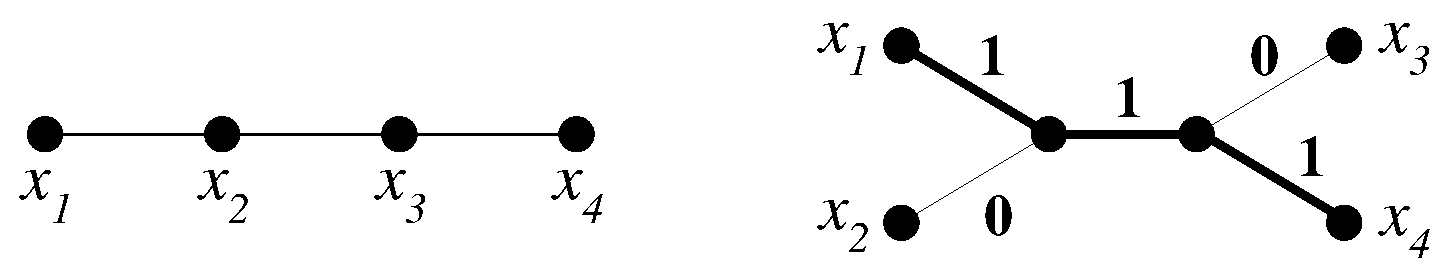
\includegraphics[width=0.15\textwidth]{quadruple.eps}
%\end{equation}
%Conversely, this quadruple explains the $P_4$. This 1-1 correspondence
%propagates to longer paths. A path of length $5$ can be viewed as a
%superposition of two paths of length $4$.  The key observation is that
%there is only a single tree with 5 leaves $x_i$, $i=1,\dots,5$ that
%displays the quadruples $x_1x_2|x_3x_4$ and $x_2x_3|x_4x_5$.  To see this,
%we apply Lemma \ref{lem:split-replace}, and conclude that a tree $T$
%displays $x_1x_2|x_3x_4$ and $x_2x_3|x_4x_5$ if and only if $T$ displays
%$x_1x_2|x_3x_4x_5$ and $x_1x_2x_3|x_4x_5$.  It is easy to see that there is
%only one such (least resolved) tree, which corresponds to the tree shown in
%Figure~\ref{fig:quintuple}.

%By induction and repeated application of Lemma \ref{lem:split-replace}, we
%conclude that a path on $n\geq 4$ vertices $x_1,\dots,x_n$ yields $n-3$
%non-trivial partial splits $x_1x_2|x_3\dots x_{n-1}x_n$,
%$x_1x_2x_3|x_4\dots x_{n-1}x_n$, \dots, $x_1x_2x_3x_4\dots
%x_{n-2}|x_{n-1}x_n$. We will refer to this set of partial splits as
%$\Sigma(P)$.

%We can now summarize the discussion above in the following
%\begin{lemma} 
%\label{lem:1path}
%Let $(T,\lambda)$ be a tree that explains $G(\Rl)/\Ro$.  If $G(\Rl)/\Ro$
%contains the path $x_1x_2\dots x_n$ then $T$ displays a ``caterpillar''
%subtree $T_n^*$ consisting of $n-2$ internal vertices $u_2u_3\dots u_{n-1}$
%forming a path with all edges labeled $1$, vertices $x_1$ and $x_n$
%adjacent to $u_2$ and $u_{n-1}$, respectively, with an edge labeled $1$,
%and $x_i$ adjacent to $u_i$ with an 0-labeled edge for $2\le i\le n-1$.
%\end{lemma}
%Figure~\ref{fig:quintuple} shows the caterpillar $T_5^*$. 

%\begin{figure}[t]
%  \begin{center}
%    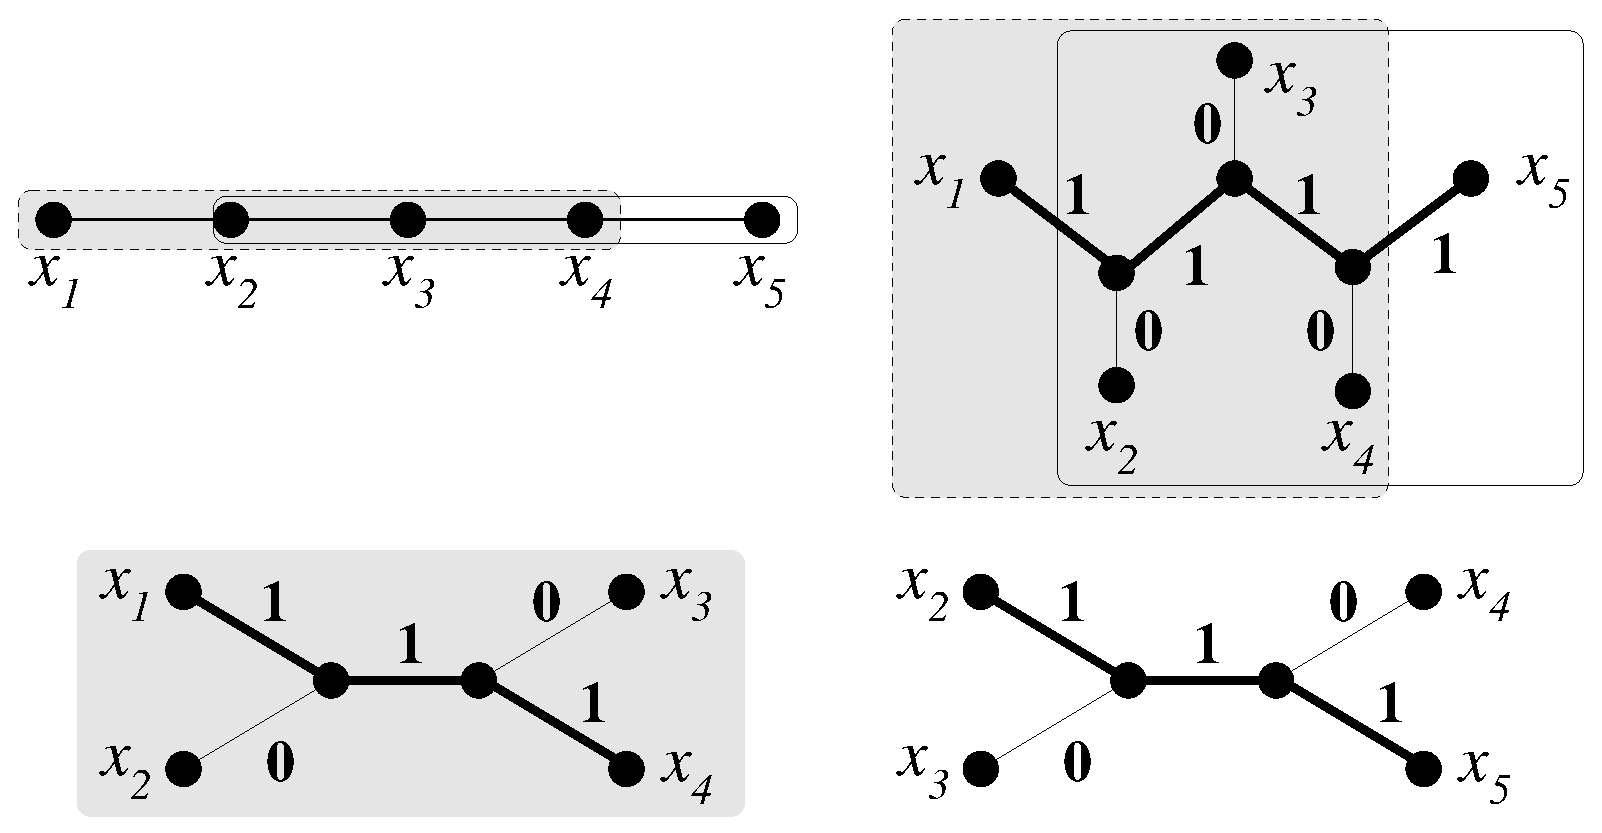
\includegraphics[width=0.15\textwidth]{quintuple.eps}
%  \end{center}
%  \caption{\remove{Paths in the $\protect\Rl$ relation imply unique split
%      systems.  The upper right edge labeled tree is the caterpillar
%      $T_5^*$.}}
%\label{fig:quintuple}
%\end{figure}
%The latter results can also be used to establish an alternative and more
%elegant proof of Lemma \ref{lem:cycle-free} and Corollary
%\ref{cor:cycle-free}.

%\begin{proof}[Alternative proof of Cor.\ \ref{cor:cycle-free}.]
%  Suppose $G(\Rl)/\Ro$ contains a minimal length cycle $C=x_1x_2\dots x_n$
%  of length $n$. We know that $n>3$ since $G(\Rl)/\Ro$ is triangle-free by
%  Lemma~\ref{lem:notriangle}. Thus suppose $n\ge 4$. Then $C$ contains the
%  two paths $x_1x_2\dots x_n$ and $x_2\dots x_nx_1$ and thus by
%  Lemma~\ref{lem:1path}, $T$ displays in particular the splits
%  $x_1x_2|x_3\dots x_n$ and $x_2x_3\dots x_{n-1}|x_n x_1$. Lemma
%  \ref{lem:split-compa} implies that these two splits are incompatible,
%% Incompatibility: 
%%  $\{1,2\}\cap\{2,3,\dots,n-1\}=\{2\}$; 
%%  $\{1,2\}\cap\{1,n\}=\{1\}$;
%%  $\{3,\dots,n-1,n\}\cap\{2,3,\dots,n-1,n\}=\{3,\dots,n-1\}$; 
%%  $\{3,\dots,n-1,n\}\cap\{1,n\}=\{n\}$.
%  and thus cannot be derived from the same tree. Therefore $G(\Rl)/\Ro$ cannot
%  contain a cycle.
%\qed\end{proof}

%\begin{figure}
%\begin{center}
%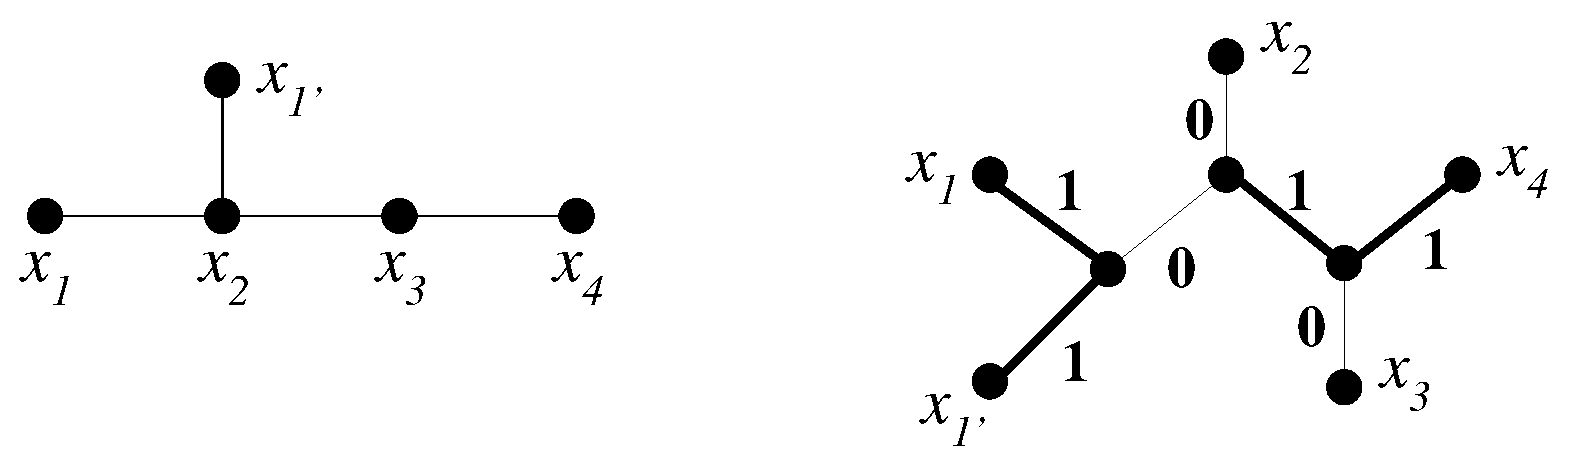
\includegraphics[width=0.15\textwidth]{quintuple2.eps}
%\end{center}
%\caption{\remove{the simplest case of overlapping paths}}
%\label{fig:quint2}
%\end{figure} 

%Partially overlapping paths can be understood in terms of individual paths
%as in Figure~\ref{fig:quint2}.  Let $Q$ be a connected component in
%$G(\Rl)/\Ro$ with vertex set $X$.  The example of Figure~\ref{fig:quint2}
%motivates to construct a \rev{phylogenetic tree $T(Q)$ with leaf set $X$}
%from the tree $Q$ as outlined in Algorithm \ref{alg:Q}.

%******* END REMOVAL old Proof *********** }

\begin{algorithm}
\caption{Compute $(T(Q), \lambda)$}
\label{alg:Q}
\begin{algorithmic}[1]
  \REQUIRE $Q$
  \ENSURE $T(Q)$
  \STATE set $T(Q)\leftarrow Q$ 
  \STATE Retain the labels of all leaves of $Q$ in $T(Q)$ and relabel 
			all interior vertices $u$ of $Q$ as $u'$.
  \STATE Label all edges of the copy of $Q$ by $\lambda(e)=1$.
  \STATE For each interior vertex $u'$ of $Q$ add a vertex $u$ to $T(Q)$ and 
		   insert the edge $uu'$. 
  \STATE Label all edges of the form $e=uu'$ with $\lambda(e)=0$. 
\end{algorithmic}
\end{algorithm}

Let $\mathbb{T}$ the set of all tree with vertex set $X$ but no edge-labels
and $\mathcal{T}$ denote the set of all edge-labeled 0-1-trees $(T,\lambda)$ with
leaf set $X$ such that each inner vertex $w\in W$ has degree at least $3$ and 
there is exactly one adjacent leaf $v$ to $w$ with $\lambda(wv)=0$ 
while all other edges $e$ in $T$ have label $\lambda(e)=1$. 

\begin{figure}
\begin{tabular}{lcr}
\begin{minipage}{0.5\textwidth}
\begin{center}
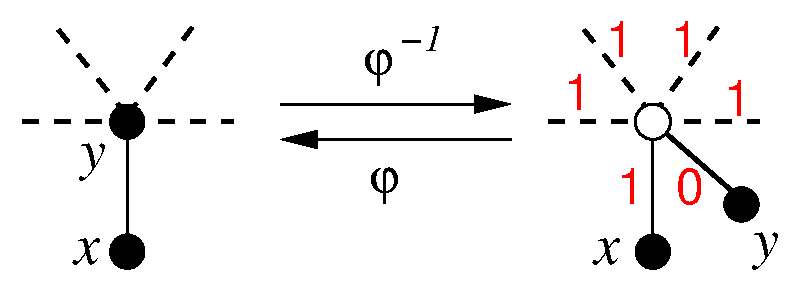
\includegraphics[width=\textwidth]{bijection.eps}
\end{center} 
\end{minipage} & & 
\begin{minipage}{0.4\textwidth}
  \caption{\rev{Illustration of the bijection $\varphi$. It contracts, at
      each interior vertex (white) of $(T,\lambda)$ the unique $0$-edge and
      transfers $y\in X$ as vertex label at the interior vertex of $Q$.
      Leafs in $(T,\lambda)$ with incident to $1$-edges remain unchanged.
      The inverse map $\varphi^{-1}$ is given by Algorithm~\ref{alg:Q}.}}
  \label{fig:bijection}
\end{minipage}
\end{tabular}
\end{figure}

\rev{
\begin{lemma}
	The map  $\varphi : \mathcal{T} \to  \mathbb{T}$ with \[\varphi: (T,\lambda)\ \mapsto Q, \] whenever
	$V(Q)=L(T)$ and  
	$Q\simeq T^*$ where $T^*$ is the underlying unlabeled tree obtained from $(T,\lambda)$ by 
	contracting all edges labeled $0$, is a bijection.
%	There is a bijection $\varphi : \mathcal{T} \to  \mathbb{T}$
%	by putting \[\varphi: (T,\lambda)\ \mapsto Q, \] if 
%	$V(Q)=L(T)$ and  
%	$Q\simeq T^*$ where $T^*$ is the underlying unlabeled tree obtained from $(T,\lambda)$ by 
%	contracting all edges labeled $0$.
	\label{lem:bijection}
\end{lemma}
\begin{proof}
	We show first that $\varphi$ and $\varphi^{-1}$ are a maps.  
	Clearly, $\varphi$ is a map, since the edge-contraction 
	is well-defined and leads to exactly one tree in $\mathbb{T}$. 
	For $\varphi^{-1}$ we construct $(T,\lambda)$ from $Q$
	as in Algorithm \ref{alg:Q}. 
	It is easy to see that  $(T,\lambda) \in  \mathcal{T}$. 
	Now consider $T^*$ obtained from  $(T,\lambda)$ by 
	contracting all edges labeled $0$. By construction, 
	$T^* \simeq Q$ (see Fig. \ref{fig:bijection}). 
	Hence,  $\varphi : \mathcal{T} \to  \mathbb{T}$ is bijective.
\end{proof}
}

\rev{The bijection is illustrated in Fig.~\ref{fig:bijection}.}


\rev{
\begin{lemma}
  Let $(T,\lambda) \in \mathcal{T}$ and $Q= \varphi((T,\lambda)) \in \mathbb{T}$.
  The set  $\mathcal{T}$	contains \emph{all} least resolved trees
  that explain $Q$. 

	Moreover, if $Q$
  is considered as a graph \mbox{$G(\Rl)/\Ro$} with vertex set $X$, then
  $(T,\lambda)$ is the unique least resolved tree that explains $Q$
	and therefore, the unique minimally resolved tree that explains $Q$.
	\label{lem:Umin}
\end{lemma}
\begin{proof}
	We start with showing that $(T,\lambda)$ explains $Q$. 
	Note, since $Q\in\mathbb{T}$, the graph $Q$ must be connected. 
	By construction and
	since $Q= \varphi((T,\lambda))$, $T^* \simeq Q$ where $T^*$ is the tree
	obtained from $T$ after contracting all 0-edges. Let $v,w\in X$ and assume
	that that there is exactly a single $1$ along the path from $v$ to $w$ in
	$(T,\lambda)$. Hence, after contracting all edges labeled $0$ we see that
	$vw\in E(T^*)$ where $T^* \simeq Q$ and thus $v\Rl w$. Note, no path between
	any two vertices in $(T,\lambda)$ can have only 0-edges (by construction).
	Thus, assume that there is more than a single 1-edge on the path between $v$
	and $w$. Hence, after after contracting all edges labeled $0$ we see that
	there is still a path in the tree $T^*$ from $v$ to $w$ with more than one
	1-edge. Since $T^* \simeq Q$, we have $vw\not \in E(Q)$ and therefore,
	$v\not\Rl w$. Thus, $(T,\lambda)$ explains $Q$. 

   By construction of the trees in $\mathcal{T}$ all 0-edges
	are incident to a leaf. Thus, by Lemma \ref{lem:contract}, 
	every least resolved tree that explains $Q$ is contained in 
 	$\mathcal{T}$. 

	It remains to show that the least resolved tree $(T,\lambda)\in \mathcal{T}$
	with $T^*\simeq Q$ that explains $Q$ is minimally resolved. 
	Assume there is another 
	least resolved tree $(T',\lambda') \in \mathcal{T}$ with leaf set $V(Q)$
   that explains $Q$. 
	By Lemma \ref{lem:bijection}, there is a bijection between those 
	$Q$ and elements in $\mathcal{T}$ for which  $T^*\simeq Q$. 
	Thus,  $T'^*\simeq Q'\not\simeq Q \simeq T^*$. However, this implies that 
	$T'\not\simeq T$. However, since in this case $(T',\lambda')$ explains $Q'$
	and  $Q'\not\simeq Q$, the pair $(T',\lambda')$ cannot explain $Q$;
	 a contradiction. 
%	We show first that 	 $(T,\lambda)$ is a least resolved  
%	tree that explains $Q$. Assume for contradiction that there is 
%	an edge $vw$ that can be contracted. First observe that neither
%	$v$ nor $w$ can be a leaf, as otherwise contraction of this edge
%	would lead to a loss of information of the particular leaf $v$, resp., $w$. 
%	Hence, both $v$ and $w$ must be inner vertices. 
%	Both $v$ and $w$ have, by construction, an adjacent leave $v'\in X$ and $w'\in X$, 
%	respectively, such that $\lambda(vv') = \lambda(ww') = 0$. However, 
%	contracting  $vw$ would immediately lead to $v'\Ro w'$; a contradiction 
%	since $\Ro$ is discrete in $Q=G(\Rl)/\Ro$. 
%	Hence, $(T,\lambda)$ is a least resolved  
%	tree that explains $Q$. 
\end{proof}	
}



\rev{As an immediate consequence of these considerations we obtain}
\begin{thm}
  Let $Q$ be a connected component in $G(\Rl)/\Ro$ with vertex set $X$.
  Then the tree $(T,\lambda)$ constructed in Algorithm~\ref{alg:Q} is the unique
  \rev{minimally} resolved tree that explains $Q$. 

\rev{	Moreover, for any pair $(T',\lambda')$ that explains $Q$, 
		the tree $T$ is obtained from $T'$ by contracting
	all \emph{inner} 0-edges and $\lambda(e) = \lambda'(e)$
	for all edges that are not contracted. }
  \label{thm:connComp}
\end{thm}
\begin{proof}
\rev{	The first statement follows from Lemma \ref{lem:contract} and \ref{lem:Umin}. 
	To see the second statement, observe that Lemma \ref{lem:contract} implies 
	that no inner 1-edge but every 0-edge can be contracted. 
	Hence, after contracting all 0-edges, no edge can be contracted and thus, 
	the resulting tree is least resolved. By Lemma \ref{lem:contract}, 
	we obtain the result.}
	\qed
\end{proof}

%\remove{old below  remove ?? 
%\begin{proof}
%  We proceed by induction on the number of vertices $|X|=n$.  For $n=1$ and
%  $n=2$ there is nothing to show, since by construction $T(Q)=Q$ and $Q$
%  must have $|X|$ leaves.  For $n=3$ we have $Q=P_3=S_2$.

%  Let us first consider stars $Q=S_m$, $m=n+1\ge 3$, in general. Denote the
%  unique central vertex by $z$ and the leaves by $u_i$. Then the
%  construction of the theorem states that $T=S_{m+1}$ and all edges $u_iz'$
%  are labeled $1$, while $\lambda(zz')=0$. The tree $T$ must have $m+1$
%  leaves because there are $m+1$ vertices in $Q$. Hence, $T=S_{m+1}$ is the
%  unique least resolved tree that could possibly produce $Q$. It is now
%  easy to check that the edge labeling indeed yields $Q$. Furthermore, no
%  other edge labeling yields $Q$. To see this, it suffices to consider
%  explicitly all cases for $n=3$ since $S_2$ is an induced subgraph of
%  $S_m$ corresponding to an induced subgraph $P_3$ of $Q$.

%  For $n=4$, we have either $Q=S_3$ or $Q=P_4$. For the latter case the
%  claim coincides with the unique quadruples of Equ.~(\ref{eq:quadruple}).
%  If the tree $Q$ is not a star and $n\ge 4$ then every vertex of $Q$ is
%  contained in at least one path on $4$ vertices.

%  Now we proceed by induction. Suppose the claim of the theorem is true for
%  all $Q$ with up to $n$ vertices. Now suppose $Q$ has $n+1\ge 5$ vertices
%  and suppose $Q$ is not a star, since we already know that the claim holds
%  for all stars. Let $q$ be a leaf of the tree $Q$. We write
%  $Q\setminus\{q\}$ for the tree obtained from $Q$ in the following way:
%  First we remove the leaf $q$ and the attached edge. If the vertex $q'$ to
%  which $q$ was attached now has degree $2$, connectedness of $Q$ implies
%  that at least one of its incident edges is a 0-edge. This edge is
%  contracted.  By assumption, the claim holds for $Q'$. Let $\bar q$ be the
%  unique neighbor of $q$ in $Q$.
% 
%  We have to distinguish two cases: either (i) $\bar q$ is not a leaf in
%  $Q'$ or (ii) $\bar q$ is a leaf in $Q'$.

%  In Case (i), the tree $T'$ contains an interior node $\bar q'$ as well as
%  a leaf $\bar q$.  Using our construction recipe to construct $T$ we add
%  $q$ to $T'$ via an edge $\bar q' q$. If $T'$ was least resolved, so is
%  $T$ since we have not added an interior vertex.  We have two
%  possibilities to label $q\bar q'$.  Of course $\lambda(q\bar q')=0$
%  immediately yields a contradiction since the path $q-\bar q'-\bar q$ then
%  would have two edges labeled $0$, but $q$ and $\bar q$ are neighbors in
%  $Q$. One easily checks that $\lambda(q\bar q')=1$ is consistent with $Q$:
%  There is exactly a single 1-edge along $q-\bar q'-\bar q$ and two or more
%  1s along the paths to any other leaf, because all other path either
%  contain an interior edge (which always is labeled $1$) or it connects to
%  another neighbor of $\bar q'$. All the latter edges, however, are also
%  labeled $1$ by our previous construction.  And instead of $\bar q'$, $q$
%  cannot be connected to any other vertex of $T(Q')$.  because of $q\Rl
%  \bar q$, connected to any interior vertex of $T(Q')$ instead of $\bar q'$
%  would either cause $q\not \Rl \bar q$ or $q\Rl p$ where $p$ is not a
%  neighbor of $q$ in $Q$.
% 
%  For Case (ii), first we show that $q$ cannot be attached to any interior
%  node of $T'$. If $q$ is attached to the interior node which is the unique
%  neighbor $q_1$ of $\bar q$ in $Q'$, then the edge $qq_1$ must be labeled
%  by 0 to have $q\Rl \bar q$. Since $q_1$ is an interior vertex, it has
%  neighbors in $Q'$. Thus $q\Rl q_2$ where $q_2$ is any neighbor of
%  $q_1$. A contradiction to $\bar q$ be the unique neighbor of $q$ in
%  $Q$. If $q$ is attached to the interior node other than $q_1$, then the
%  path of $q$ to $\bar q$ in $Q$ will has at least two edges labeled by 1,
%  a contradiction to $q \Rl \bar q$.
%  
%  As a consequence of the results on paths above we know that for every
%  path $P_4$ $q-\bar q-u-v$ in $Q$ the tree $T$ must display the quadruple
%  $q\bar q|uv$. On the other hand, since $\bar q$ is a leaf in $Q'$, $u$
%  and $q$ are its only neighbors in $Q$ and thus $q\bar q|rs$ is a
%  quadruple displayed by $T$ for all $\{r,s\}\ne\{q,\bar q\}$ in
%  $T$. Therefore $q$ and $\bar q$ form a cherry in $T$, i.e., there must be
%  an interior vertex $\bar q'$ that has both $q$ and $\bar q$ as its
%  neighbors. Furthermore $\bar q'$ is necessarily connected to the rest of
%  $T$ by an interior edge. From the quadruple $q\bar q|uv$ corresponding to
%  the path $q-\bar q-u-v$, furthermore, we conclude that the interior edge
%  must connect $\bar q'$ with $u'$. It is clear that the resulting tree is
%  least resolved: None of the new edges $q\bar q'$, $\bar q\bar q'$, $\bar
%  q'u'$ can be contracted without contradiction, and all edges in the
%  remainder of the tree all edges are necessary due to the induction
%  hypothesis. Therefore the tree $T$ is uniquely defined by $Q$.

%  Let us now turn to the labeling of $T$. First we note that exactly one of
%  the edge $q\bar q'$ or $q'\bar q'$ must be labeled 1. Furthermore there
%  must be a single 1-edge along the paths $\bar q-\bar q'-u' -u$ and two or
%  more 1's along $q-\bar q'-u' -u$. Therefore $\lambda(q\bar q')=1$ and
%  $\lambda(q'\bar q')=0$. Using the known constraints within $T'$ as argued
%  previously we see that $\lambda(uu')=0$, and thus $\lambda(\bar
%  q'u')=1$. Hence, the labeling of $T$ is again unique and coincides with
%  the labeling described in the claim of the theorem.  

%  We therefore conclude that for all connected components $Q$ both the
%  least resolved tree and its labeling is uniquely determined.  \qed
%\end{proof}
%}

We are now in the position to demonstrate how to obtain a least resolved
tree that explains $G(\Rl)/\Ro$ also in the case that $G(\Rl)/\Ro$ itself
is not connected. To this end, denote by $Q_1,\dots Q_k$ the connected
components of $G(\Rl)/\Ro$. We can construct a \rev{phylogenetic tree
  $T(G(\Rl)/\Ro))$ with leaf set $X$} for $G(\Rl)/\Ro$ using Alg.\
\ref{alg:all}. It basically amounts to constructing a star $S_k$ with
interior vertex $z$, where its leaves are identified with the trees
$T(Q_i)$.

\begin{algorithm}
\caption{Compute $(T(G(\Rl)/\Ro)), \lambda)$}
\label{alg:all}
\begin{algorithmic}[1]
  \REQUIRE disconnected $G(\Rl)/\Ro)$
  \ENSURE $T(G(\Rl)/\Ro))$	
  \STATE $T(G(\Rl)/\Ro)) \gets (\{z\},\emptyset)$
  \FOR{For each connected component $Q_i$}
     \STATE	construct $(T(Q_i), \lambda_i)$ with Alg.\ \ref{alg:Q}
		and add to $T(G(\Rl)/\Ro))$.
     \IF{$T(Q_i)$ is the single vertex graph $(\{x\},\emptyset)$}
	\STATE add edge $zx$
     \ELSIF{$T(Q_i)$ is the edge $v_iw_i$}
        \STATE remove the edge
                $v_iw_i$ from $T(Q_i)$, insert a vertex $x_i$ in $T(Q_i)$
                and the edges $x_iv_i$, $x_iw_i$. 
        \STATE  set either $\lambda_{i}(x_iv_i)=1$ and $\lambda(x_iw_i)=0$
		or $\lambda_{i}(x_iv_i)=0$ and $\lambda(x_iw_i)=1$. 
                \label{step:edge}
	\STATE  add edge $zx_i$ to $T(G(\Rl)/\Ro))$.
     \ELSE \STATE \label{item:z}  	
                add edge edge $zq'_i$ to  $T(G(\Rl)/\Ro))$
		for an arbitrary interior vertex $q'_i$ of $T(Q_i)$. 
     \ENDIF		 
   \ENDFOR
   \STATE       Set $\lambda(zv)=1$ for all edges $zv$ and 
		$\lambda(e)=\lambda_i(e)$ for all edges $e\in T(Q_i)$.	
\end{algorithmic}
\end{algorithm}

\begin{thm}
  Let $Q_1,\dots Q_k$ be the connected components in $G(\Rl)/\Ro$.  Up to
  the choice of the vertices $q'_i$ in Line \ref{item:z} of Alg.\
  \ref{alg:all}, the tree $T^* = T(G(\Rl)/\Ro))$ is a \rev{minimally
    resolved tree that explains $G(\Rl)/\Ro$. It is unique up to the choice
    of the $zq'_i$ in Line \ref{item:z}.}
  \label{thm:star-tree}
\end{thm}
\begin{proof}
 \rev{ Since every tree $T(Q_i)$ explains a connected component in $G(\Rl)/\Ro$,
  from the construction of $T^*$ it is easily seen that $T^*$ explains
  $G(\Rl)/\Ro$.  Now we need to prove that $T^*$ is a minimally resolved
  tree that explains $G(\Rl)/\Ro$.

  To this end, consider an arbitrary tree $T'$ that explains $G(\Rl)/\Ro$.
  Since $T'$ explains $G(\Rl)/\Ro$, it must explain each of the connected
  components $Q_1,\dots Q_k$. Thus, each of the subtrees $T'_i$ of $T'$
  with leaf set $V(Q_i)$ that are minimal w.r.t.\ inclusion must explain
  the connected component $Q_i$, $1\le i \le k$.  Note the $T'_i$ may have
  vertices of degree 2.

  We show first that $T(Q_i)$ is obtained from $T'_i$ by contracting all
  inner 0-edges and all 0-edges of degree 2.  If there are no vertices of
  degree 2, we can immediately apply Thm.\ \ref{thm:connComp}.

  If there is a vertex $v$ of degree 2, then $v$ cannot be incident to two
  1-edges, as otherwise the relation explained by $T'_i$ would not be
  connected, contradicting the assumption that $T'_i$ explains the
  connected component $Q_i$.  Thus, if there is a vertex $v$ of degree 2 it
  must be incident to a 0-edge $vw$.  Contracting $vw$ preserves the
  property of $\Ro$ being discrete.  If $w$ is a leaf, we can contract the
  edge $vw$ to a new leaf vertex $w$; if $vw$ is an inner edge we simply
  contract it to some new interior vertex. In both cases, we can argue
  analogously as in the proof of Lemma \ref{lem:contract} that the tree
  obtained from $T'_i$ after contracting $vw$, still explains $Q_i$.  This
  procedure can be repeated until no degree two vertices are in the
  contracted $T'_i$.

  In particular, the resulting tree is a phylogenetic tree that explains
  $Q_i$. Now we continue to contract all remaining inner 0-edges and apply
  Thm.\ \ref{thm:connComp} to conclude that we obtain $T(Q_i)$.

  We continue to show that two distinct subtrees $T'_i$, and $T'_j$ do not
  have a common vertex in $T'$.  If one of $Q_i$ or $Q_j$ is a single
  vertex graph, then $T'_i$ or $T'_j$ consists of a single leaf only, and
  the statement holds trivially.

  Hence, assume that both $Q_i$ and $Q_j$ have at least three vertices.
  Lemma \ref{lem:contract} implies that each inner vertex of the minimally
  resolved trees $T(Q_i)$ and $T(Q_j)$ is incident to exactly one 0-edge as
  long as $Q_i$ is not an edge.  Since $T(Q_i)$ can be obtained from $T'_i$
  by the procedure above, for each inner vertex $v$ in $T'_i$ there is a
  leaf $x$ in $T'_i$ such that the unique path from $v$ to $x$ contains
  only 0-edges.  The same arguments apply, if $Q_i$ is an edge $xy$. In
  this case, the tree $T'_i$ must have $x$ and $y$ as leaves, which implies
  that $T'_i$ has at least one inner vertex $v$ and that there is exactly
  one 1-edge along the path from $x$ to $y$. Thus, for each inner vertex in
  $T'_i$ there is a path to either $x$ or $y$ that that contains only
  0-edges.

  Let $v$ and $w$ be an arbitrary inner vertices of $T'_i$ and $T'_j$,
  respectively, and let $x$ and $y$ be leafs that are connected to $v$ and
  $w$, resp., by a path that contains only 0-edges. If $v=w$, then $x\Ro
  y$, contradicting the property of $\Ro$ being discrete.  Thus, $T'_i$ and
  $T'_j$ cannot have a common vertex in $T'$.  Moreover, there is no edge
  $vw$ in $T'$, since otherwise either $x\Ro y$ (if $\lambda(vw)=0$) or
  $x\Rl y$ (if $\lambda(vw)=1$).  Hence, any two distinct vertices in
  $T'_i$ and $T'_j$ have distance at least two in $T'$.

  This implies that the construction as in Alg.\ \ref{alg:all} yields a
  least resolved tree.  In more detail, since the subtrees explaining $Q_i$
  in any tree that explains $G(\Rl)/\Ro$ must be vertex disjoint, the
  minimally resolved trees $T(Q_1),\dots,T(Q_k)$ must be subtrees of any
  minimally resolved tree that explain $G(\Rl)/\Ro$, as long as all $Q_i$
  are single vertex graphs or have at least one inner vertex.

  If $Q_i$ is a single edge $v_iw_i$ and thus $T(Q_i) = v_iw_i$ where
  $\lambda(v_iw_i)=1$, we modify $T(Q_i)$ in Line \ref{step:edge} to obtain
  a tree isomorphic to $S_2$ with inner vertex $x_i$. This modification is
  necessary, since otherwise (at least one of) $v_i$ or $w_i$ would be an
  inner vertex in $T^*$, and we would loose the information about the
  leaves $v_i,w_i$. In particular, we need to add this vertex $x_i$ because
  we cannot attach the leaves $v_i$ (resp.\ $w_i$) by an edge $x_jv_i$
  (resp.\ $x'_jw_i$) to some subtree subtree $T(Q_j)$.  To see this, note
  that at least one of the edges $x_jv_i$ and $x'_jw_i$ must be a
  0-edge. However, $x_j$ and $x'_j$ are already incident to a 0-edge
  $x_jv'_i$ or $x'_jw'_i$ (cf.\ Lemma \ref{lem:contract}), which implies
  that $\Ro$ would not be discrete; a contradiction.  By construction, we
  still have $v_i\Rl w_i$ in Line \ref{step:edge}.
	
  Finally, any two distinct vertices in $T(Q_i)$ and $T(Q_j)$ have distance
  at least two in $T^*$, as shown above. Hence, any path conntecting two
  two subtrees $T(Q_i)$ in $T^*$ contains and least two edges and hence at
  least one vertex that is not contained in any of the $T(Q_i)$. Therefore,
  any tree explaining $Q$ has at least $1+\sum_i |V(T(Q_i))|$ vertices.

  We now show that a single addition vertex $z$, which we may consider as a
  trivial tree $(\{z\},\emptyset)$, is sufficient. Indeed, we may connect
  the different trees to $z$ by insertion of an edge $zq'_i$, where $q'_i$
  is an arbitrary inner vertex of $T(Q_i)$ and label these edges
  $\lambda(zq'_i)=1$.  Thus, no two leaves $u$ and $w$ of distinct trees
  are either in relation $\Ro$ or $\Rl$, as required. The resulting trees 
  have the minimal possible number of vertices, i.e., they are minimally
  resolved. 
  \qed}
\end{proof}

\subsection*{Binary trees}

Instead of asking for least resolve trees that explain $G(\Rl)/\Ro$, we may
also consider the other extreme and ask which binary, i.e., fully resolved
tree can explain $G(\Rl)/\Ro$. Recall that an $X$-tree is called binary or
fully resolved if the root has degree $2$ while all other interior vertices
have degree $3$.  From the construction of the least resolved trees we
immediately obtain the following:
\begin{cor}
  A least resolved tree $T(Q)$ for a connected component $Q$ of
  $G(\Rl)/\Ro$ is binary if and only if $Q$ is a path.
\end{cor}

If a least resolved tree $T(Q)$ of $G(\Rl)/\Ro$ is a star, we have:
\begin{lemma}\label{lem:star}
  If a least resolved tree $T(Q)$ explaining $G(\Rl)/\Ro$ is a star
  with $n$ leaves, then either
  \begin{itemize}
    \item[(a)] all edges in $T(Q)$ are 1-edges and $Q$ has no edge, or 
    \item[(b)] there is exactly one 0-edge in $T(Q)$ and $Q$ is a star
        with $n-1$ leaves.
    \end{itemize}
  \end{lemma}
\begin{proof}
  For implication in case (a) and (b) we can re-use exactly the same
  arguments as in the proofs of Theorem \ref{thm:connComp} and
  \ref{thm:star-tree}.

  Now suppose there are at least two (incident) 0-edges in $T(Q)$, whose
  endpoints are the vertices $u$ and $v$. Then $u\Ro v$, which is
  impossible in $G(\Rl)/\Ro$.  \qed
\end{proof}

To construct the binary tree representing the star $Q=S_n$, we consider the
set of all binary trees with $n$ leaves and 0/1-edge labels. If $S_n$ is of
type (a) in Lemma~\ref{lem:star}, then all terminal edges are labeled $1$
and all interior edges are arbitrarily labeled $0$ or $1$.
Figure~\ref{fig:non_lrt} shows an example for $S_6$.  If $S_n$ is of type
(b), we label the terminal edges in the same way as in $T(Q)$ and all
interior edge are labeled 0. In this case, for each binary tree there is
exactly one labeling.

\begin{figure}[htbp]
\begin{center}
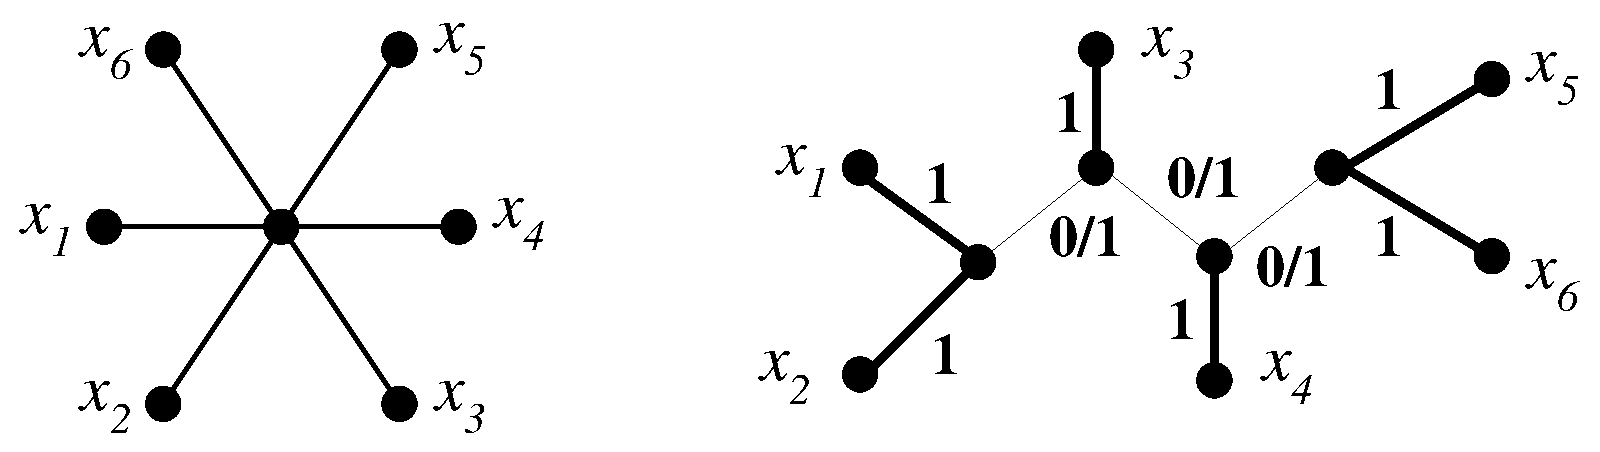
\includegraphics[width=0.6\textwidth]{non_lrt-new.eps}
\end{center}
\caption{For fixed underlying tree $T(Q)$, in this case a star $S_6$ with
  all $1$, there are in general multiple labelings $\lambda$ that represent
  the same relation $Q$, here the empty relation.}
\label{fig:non_lrt}
\end{figure}

 

In order to obtain the complete set of binary trees that explain $G$ we can
proceed as follows. If $G$ is connected, there is a single least resolved
tree $T(G)$ explaining $G$. If $G$ is not connected then there are multiple
least resolved trees $T$. They are described by
Thm.~\ref{thm:star-tree}. For every such least resolved tree $T$ we iterate
over all vertices $v_0$ of $T$ with degree $k>3$ and perform the following
manipulations:
\begin{itemize}
\item[{1.}] Given a vertex $v_0$ of $T$ with degree $k>3$, denote its
  neighbors by $v_1, v_2,\dots, v_k$. Delete vertex $v_0$ and its attached
  edges from $T$, and rename the neighbors $v_i$ to $v_i'$ for all $1\leq
  i\leq k$. Denote the resulting forest by $F(v_0)$.
\item[{2.}] Generate all binary trees with leaves $v_2,\dots, v_k$ as
  described in the previous paragraph.
  \TODO{how are the edges in these trees labeled}
\item[{3.}] Each of these binary trees is inserted into a copy of the
  forest $F(v_0)$ by \rev{identifying} $v_i$ and $v_i'$ for all $1\leq
  i\leq k$.
\end{itemize}
For a given least resolved tree $T$ this yields the set of all
$\prod_{v_0} t(\mathrm{deg}(v_0))$ pairwise distinct binary trees, where
$t(k)$ denotes the number of binary trees with $k$ leaves. The union of
these tree sets is then the set of all binary trees explaining $G$.  To
establish the correctness of this procedure, we prove
\newline
\begin{lemma}\label{lem:binary}
  The procedure outlined above generates all binary trees representing $Q$.
\end{lemma}
\begin{proof}
  It is easy to check that the trees we get are indeed binary trees, and
  any binary tree we get represents $Q$.
 
  On the other hand, by Theorem~\ref{thm:star-tree} we know that the least
  resolved tree representing $Q$ is $T(Q)$.  By the definition of least
  resolved tree, here are two ways to get all the trees from least resolved
  tree. Add 0 interior edges, or add 1 interior edges in proper place.
  Thus if the least resolved tree has degree 2 vertices, then by adding
  interior edges we cannot change the degree of degree 2 vertices, so that
  we cannot get a binary tree.  In this case there is no binary tree
  representation.  Otherwise, whenever adding an extra vertex, we need to
  attach the vertex an edge, where we can only move the edges from the
  neighborhood.  The construction goes over all the possibilities so that
  it gets all the binary tree with this least resolved tree. \qed
\end{proof}

By the proof of Lemma~\ref{lem:binary} we immediately obtain the following
Corollary that characterizes the condition that $Q$ cannot be explained by
a binary tree.
\begin{cor}
  $G(\Rl)/\Ro$ cannot be explained by a binary tree if and only if
  $G(\Rl)/\Ro$ \rev{is a forest with} exactly two connected components.
\end{cor}
The fact that exactly two connected components appear as a special case is
the consequence of a conceptually too strict definition of ``binary
tree''. If we allow a single ``root vertex'' of degree $2$ in this special
case, we no longer have to exclude two-component graphs.

\section{The antisymmetric single-1 relation}
\label{sect:1dir}

The antisymmetric version $x\Rld y$ of the 1-relation shares many basic
properties with its symmetric cousin. We therefore will not show all formal
developments in full detail. Instead, we will where possible appeal to the
parallels between $x\Rld y$ and $x\Rl y$. For convenience we recall the
definition: $x \Rld y$ if and only if all edges along $\mathbb{P}(u,x)$ are
labeled $0$ and exactly one edge along $\mathbb{P}(u,y)$ is labeled $1$,
where $u=\lca{x,y}$. As an immediate consequence we may associate with
$\Rld$ a symmetrized 1-relation $x\Rl y$ whenever $x\Rld y$ or $y\Rld
x$. Thus we can infer (part of) the underlying unrooted tree topology by
considering the symmetrized version $\Rl$. On the other hand, $\Rld$ cannot
convey more information on the unrooted tree from which $\Rld$ and its
symmetrization $\Rl$ are derived. It remains, however, to infer the
position of the root from directional information. Instead of the
quadruples used for the unrooted trees in the previous section, structural
constraints on rooted trees are naturally expressed in terms of triples.


In the previous section we have considered $\Rl$ in relation to unrooted
trees only. Before we start to explore $\Rld$ we first ask whether $\Rl$
contains any information about the position of the root and if it already
places any constraints on $\Rld$ beyond those derived for $\Rl$ in the
previous section. In general the answer to this question will be negative,
as suggested by the example of the tree $T_5^*$ in Figure
\ref{fig:root}. Any of its inner vertex can be chosen as the root, and
each choice of a root vertex yields a different relation $\Rld$.

Nevertheless, at least partial information on $\Rld$ can be inferred
uniquely from $\Rl$ and $\Ro$. Since all connected components in
$G(\Rl)/\Ro$ are trees, we observe that the underlying graphs
$\underline{G(\Rld)/\Ro}$ of all connected components in $G(\Rld)/\Ro$ must
be trees as well.  Moreover, since $\Ro$ is discrete in $G(\Rl)/\Ro$, it is
also discrete in $G(\Rld)/\Ro$.

Let $Q$ be a connected component in $\underline{G(\Rld)/\Ro}$.  \TODO{If
  $Q$ is an isolated vertex or a single edge there is nothing to show.} In
either case there is only a single tree and the position of its root in
uniquely determined. Thus we assume that $Q$ contains at least three
vertices from here on. By construction, any three vertices $x,y,z$ in a
connected component $Q$ in $G(\Rld)/\Ro$ either induce a disconnected
graph, or a tree on three vertices.  Let $x,y,z\in V(Q)$ induce such a
tree. Then there are three possibilities (up to relabeling of the vertices)
for the induced subgraph contained in $G(\Rld)/\Ro = (V,E)$:
\begin{itemize}
\item[(i)] $xy, yz \in E$ implying that $x\Rld y \Rld z$, 
\item[(ii)] $yx, yz \in E$ implying that $y\Rld x$ and $y \Rld z$,
\item[(iii)] $xy, zy \in E$ implying that $x\Rld y$ and $z \Rld y$. 
\end{itemize}
Below, we will show that Cases (i) and (ii) both imply a unique tree on the
three leaves $x,y,z$ together with a unique 0/1-edge labeling for the
unique resolved tree $T(Q)$ that displays $Q$, see Fig.\
\ref{fig:2cases}. Moreover, we shall see that Case (iii) cannot occur.

\begin{figure}[t]
\begin{center}
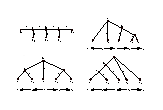
\includegraphics[width=\textwidth]{fig4.eps}
\end{center}
\caption{Placing the root. For the tree $T_5^*$ of Fig.\
  \ref{fig:quintuple} each of the tree inner vertices $a$, $b$, or $c$ can
  be chosen as the root, giving rise to three distinct relations $\Rld$.
  For the ``siblings'' in the unrooted tree $x_1,x_2$ as well as $x_4,x_5$
  it holds that $x_2\Rld x_1$ and $x_4\Rld x_5$ for all three distinct
  relations.  Thus, there are uniquely determined parts of $\Rld$ conveyed
  by the information of $\Ro$ and $\Rl$ only.}
\label{fig:root}
\end{figure} 
\begin{figure}[t]
\begin{center}
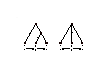
\includegraphics[width=0.6\textwidth]{fig5.eps}
\end{center}
\caption{There are only two possibilities for induced connected subgraphs
  $H$ in $G(\Rld)/\Ro$ on three vertices, cf.\ Lemma \ref{lem:case-i},
  \ref{lem:case-ii}, and \ref{lem:case-iii}.  Each of the distinct induced
  subgraphs imply a unique least resolved tree with a unique labeling.}
\label{fig:2cases}
\end{figure} 

\begin{lemma}
  In Case (i), the unique triple $\rt{yz|x}$ must be displayed by
  any tree $T(Q)$ that explains $Q$.  Moreover, the paths $\P(u,v)$ and
  $\P(v,z)$ in $T(Q)$ contain both exactly one 1-edge, while the other
  paths $\P(u,x)$ and $\P(v,y)$ contain only 0-edges, where
  $u=\lca{xy}=\lca{xz} \neq \lca{yz}=v$.
  \label{lem:case-i}
\end{lemma}
\begin{proof}
  Let $x,y,z\in V(Q)$ such that $xy, yz \in E$ and thus, $x\Rld y \Rld z$.
  Notice first that there must be two distinct last common ancestors for
  pairs of the three vertices $x,y,z$; otherwise, if
  $u=\lca{xy}=\lca{xz} = \lca{yz}$, then the path $\P(uy)$ contains a
  1-edge (since $x\Rld y$) and hence $y\Rld z$ is impossible.  We
  continue to show that $u=\lca{xy}=\lca{xz}$.  Assume that $u=\lca{xy}\neq
  \lca{xz}$.  Hence, either the triple $\rt{xz|y}$ or $\rt{xy|z}$ is
  displayed by $T(Q)$. In either case the path $\P(u,y)$ contains a 1-edge,
  since $x\Rld y$. This, however, implies $y\not\Rld z$, a contradiction.
  Thus, $u=\lca{xy} = \lca{xz}$. Since there are two distinct last common
  ancestors, we have $u\neq v=\lca{yz}$.  Therefore, the triple $\rt{yz|x}$
  must be displayed by $T(Q)$. From $y\Rld z$ we know that  $\P(v,y)$ only
  contains 0-edges and $\P(v,z)$ contains exactly one 1-edge;  $x\Rld y$
  implies that $\P(x,u)$ contains only 0-edges.  Moreover, since $\P(x,y) =
  \P(x,u)\cup \P(u,v)\cup \P(v,y)$ and $x\Rld y$, the path $\P(u,v)$ must
  contain exactly one 1-edge.  
  \qed
\end{proof}

\begin{lemma}
  In Case (ii), there is a unique tree on the three vertices $x,y,z$
  with single root $\rho$ displayed by any least resolved tree $T(Q)$ that
  explains $Q$.  Moreover, the path $\P(\rho,y)$ contains only 0-edges,
  while the other paths $\P(\rho,x)$ and $\P(\rho,z)$ must both contain
  exactly one 1-edge.
  \label{lem:case-ii}
\end{lemma}
\begin{proof}
  Assume for contradiction that there is a least resolved tree $T(Q)$
  that displays $\rt{xy|z}$, $\rt{yz|x}$, or $\rt{xz|y}$. 

  The choice of $\rt{xy|z}$ implies $u=\lca{xy}\neq \lca{xz}=\lca{yz}=v$.
  Since $y\Rld x$ and $y\Rld z$, $\P(v,y) \subsetneq \P(u,y)$ contain only
  0-edges, while $\P(u,x)$ and $\P(v,z)$ each must contain exactly one
  1-edge, respectively.  This leads to a tree $T'$ that yields the correct
  $\Rld$-relation.  However, this tree is not least resolved.  By
  contracting the path $\P(u,v)$ to a single vertex $\rho$ and maintaining
  the labels on $\P(\rho,x)$, $\P(\rho,y)$, and $\P(\rho,z)$ we obtain the
  desired labeled least resolved tree with single root.
	
  For the triple $\rt{yz|x}$ the existence of the unique, but not least
  resolved tree can be shown by the same argument with exchanged roles of
  $x$ and $y$.
	
  For the triple $\rt{xz|y}$ we $u = \lca{xy} = \lca{yz} \neq \lca{xz} =
  v$. From $y\Rld x$ and $y\Rld z$ we see that both paths $\P(u,x) =
  \P(u,v)\cup \P(v,x)$ and $\P(u,z) = \P(u,v)\cup \P(v,z)$ contain exactly
  one 1-edge, while all edges in $\P(u,y)$ are labeled $0$.  There are two
  cases: (1) The path $\P(u,v)$ contains this 1-edge, which implies that
  both paths $\P(v,x)$ and $\P(v,z)$ contain only 0-edges. But then $x\Ro
  z$, a contradiction to $\Ro$ being discrete.  (2) The path $\P(u,v)$
  contains only 0-edges, which implies that each of the paths $\P(v,x)$ and
  $\P(v,z)$ contain exactly one 1-edge. Again, this leads to a tree that
  yields the correct $\Rld$-relation, but it is not least resolved.  By
  contracting the path $\P(u,v)$ to a single vertex $\rho$ and maintaining
  the labels on $\P(\rho,x)$, $\P(\rho,y)$, and $\P(\rho,z)$ we obtain the
  desired labeled least resolved tree with single root.  \qed
\end{proof}

\begin{lemma}
  Case (iii) cannot occur.
  \label{lem:case-iii}
\end{lemma}
\begin{proof}
  Let $x,y,z\in V(Q)$ such that $xy, zy \in E$ and thus, $x\Rld y$ and $z
  \Rld y$.  Hence, in the rooted tree that represents this relationship we
  have the following situation: All edges along $\mathbb{P}(u,x)$ are
  labeled $0$; exactly one edge along $\mathbb{P}(u,y)$ is labeled $1$,
  where $u=\lca{x,y}$; all edges along $\mathbb{P}(v,z)$ are labeled $0$,
  and exactly one edge along $\mathbb{P}(v,y)$ is labeled $1$, where
  $v=\lca{y,z}$.  Clearly, $\lca{x,y,z}\in \{u,v\}$.  If $u=v$, then all
  edges in $\mathbb{P}(u,x)$ and $\mathbb{P}(u,z)$ are labeled $0$,
  implying that $x\Ro y$, contradicting that $\Ro$ is discrete.
	
  Now assume that $u=\lca{x,y}\neq v=\lca{y,z}$.  Hence, one of the triples
  $\rt{xy|z}$ or $\rt{yz|x}$ must be displayed by $T(Q)$.  W.l.o.g., we can
  assume that $\rt{yz|x}$ is displayed, since the case $\rt{xy|z}$ is shown
  analogously by interchanging the role of $x$ and $z$.  Thus, $\lca{x,y,z}
  = \lca{x, y} = u\neq \lca{yz}=v$. Hence, $\mathbb{P}(u,y) =
  \mathbb{P}(u,v) \cup \mathbb{P}(v,y)$.  Since $z\Rld y$, the path
  $\mathbb{P}(v,y)$ contains a single 1-edge and $\mathbb{P}(v,z)$ contains
  only 0-edges. Therefore, the paths $\mathbb{P}(u,x)$ and
  $\mathbb{P}(u,v)$ contain only 0-edges, since $x\Rl y$.  Since
  $\mathbb{P}(x,z) = \mathbb{P}(x,u)\cup \mathbb{P}(u,v)\cup
  \mathbb{P}(v,z)$ and all edges along $\mathbb{P}(u,x)$, $\mathbb{P}(u,v)$
  and $\mathbb{P}(v,z)$ are labeled $0$, we obtain $x\Ro z$, again a
  contradiction.\qed
\end{proof}

Taken together, we obtain the following immediate implication:
\begin{cor}
  The graph $G(\Rld)/\Ro$ does not contain a pair of edges of the form $xv$
  and $yv$.
\label{cor:edge-pointing}
\end{cor}

Recall that the connected components $\underline{Q}$ in $G(\Rld)/\Ro$ are
trees. By Cor.\ \ref{cor:edge-pointing}, $Q$ must be composed of
distinct paths that ``point away'' from each other.  In other words,
  let $P$ and $P'$ be distinct directed path in $Q$ that share a vertex
  $v$, then it is never the case that there is an edge $xv$ in $P$ and an
  edge $yv$ in $P'$, that is, both edges ``pointing'' to the same vertex
  $v$. We first consider directed paths in isolation.

\begin{lemma}
  Let $Q$ be a connected component in $G(\Rld)/\Ro$ that is a
  directed path with $n\ge 3$ vertices labeled $x_1,\dots,x_n$ such that
  $x_ix_{i+1}\in E(Q)$, $1\leq i\leq n-1$. 
  Then the tree $T(Q)$ explaining $Q$ must display all triples in $\mathcal
  R_Q = \{\rt{x_ix_j|x_l} \mid i,j>l\geq 1\}$.  Hence, $T(Q)$ must display
  $\binom{n}{3}$ triples and is therefore the unique (least resolved)
  binary rooted tree $(\dots(x_n,x_{n-1})x_{n-2})\dots)x_2)x_1$ that
  explains $Q$.  Moreover, all inner edges in $T(Q)$ and the edge incident
  to $x_n$ are labeled $1$ while all other edges are labeled $0$.
  \label{lem:path-tree}
\end{lemma}
\begin{proof}
  Let $Q$ be a directed path as specified in the lemma. We prove the
  statement by induction. For $n=3$ the statement follows from Lemma
  \ref{lem:case-i}. Assume the statement is true for $n=k$. Let $Q$ be a
  directed path with vertices $x_1,\dots,x_k, x_{k+1}$ and edges
  $x_ix_{i+1}$, $1\leq i\leq k$ and let $T(Q)$ be a tree that explains
  $Q$. For the subpath $Q'$ on the vertices $x_2,\dots,x_{k+1}$ we can
  apply the induction hypothesis and conclude that $T(Q')$ must display the
  triples $\rt{x_ix_j|x_l}$ with $i,j>l\geq 2$ and that all inner edges in
  $T(Q')$ and the edge incident to $x_{k+1}$ are labeled $1$ while all
  other edges are labeled $0$. Since $T(Q)$ must explain in particular the
  subpath $Q'$ and since $T(Q')$ is fully resolved, we can conclude that
  $T(Q')$ is displayed by $T(Q)$ and that all edges in $T(Q)$ that are also
  in $T(Q')$ retain the same label as in $T(Q')$ .
	
  Thus $T(Q)$ displays in particular the triples $\rt{x_ix_j|x_l}$ with
  $i,j>l\geq 2$.  By Lemma \ref{lem:case-i}, and because there are edges
  $x_1x_2$ and $x_2x_3$, we see that $T(Q)$ must also display
  $\rt{x_2x_3|x_1}$.  Take any triple $\rt{x_3x_j|x_2}$, $j>3$.
  Application of the triple-inference rules shows that any tree that
  displays $\rt{x_2x_3|x_1}$ and $\rt{x_3x_j|x_2}$ must also display
  $\rt{x_2x_j|x_1}$ and $\rt{x_3x_j|x_1}$. Hence, $T(Q)$ must display these
  triples.  Now we apply the same argument to the triples $\rt{x_2x_j|x_1}$
  and $\rt{x_ix_j|x_2}$, $i,j>2$ and conclude that in particular, the
  triple $\rt{x_ix_j|x_1}$ must be displayed by $T(Q)$ and thus, the the
  entire set of triples $\{\rt{x_ix_j|x_l} \colon i,j>l\geq 1\}$.  Hence,
  there are $\binom{n}{3}$ triples and thus, the set of triples that needs
  to be displayed by $T(Q)$ is strictly dense. Making use of a technical
  result from \cite[Suppl. Material]{Hellmuth:15a}, we obtain that $T(Q)$
  is the unique binary tree $(\dots(x_n,x_{n-1})x_{n-2})\dots)x_2)x_1$. Now
  it is an easy exercise to verify that the remaining edge containing $x_1$
  must be labeled $0$, while the inner edge not contained in $T(Q')$ must
  all be 1-edges.\qed
\end{proof}

\begin{figure}
\begin{center}
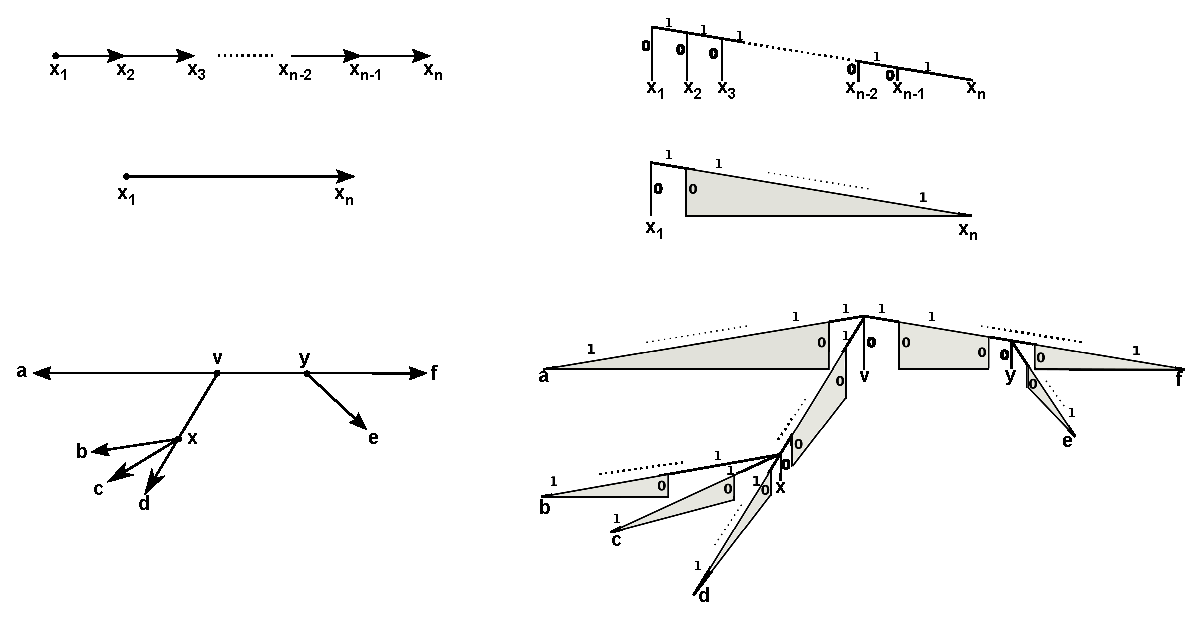
\includegraphics[width=1.\textwidth]{di-path-tree.eps}
\end{center}
\caption{Connected components $Q$ in $G(\Rld)/\Ro$ are trees composed of
  paths pointing away from each other.  On the top, a directed path
  $\mathbb P(x_1,x_n)$ together with its unique least resolved tree
  representation is shown. In the middle, an abstract picture of the path
  $\mathbb P(x_1,x_n)$ and its tree is given.  Bottom, a larger example of
  a connected component $Q$ in $G(\Rld)/\Ro$ and its tree-representation
  are sketched.}
\label{fig:Qtree}
\end{figure}

If $Q$ is connected but not a simple path, it is a tree composed of the
paths pointing away from each other as shown in Fig. \ref{fig:Qtree}. It
remains to show how to connect the distinct trees that explain these paths
to obtain a tree $T(Q)$ for $Q$.  To this end, we show first that there is
a unique vertex $v$ in $Q$ such that no edge ends in $v$.

\begin{lemma}
  Let $Q$ be a connected component in $G(\Rld)/\Ro$.  Then there is a
  unique vertex $v$ in $Q$ such that there is no edge $xv\in E(Q)$.
  \label{lem:unique-v}
\end{lemma}
\begin{proof}
  Corollary \ref{cor:edge-pointing} implies that for each vertex $v$ in $Q$
  there is at most one edge $xv\in E(Q)$.  If for all vertices $w$ in $Q$
  we would have an edge $xw\in E(Q)$, then $Q$ contains cycles,
  contradicting the tree structure of $Q$. Hence, there is at least one
  vertex $v$ so that there is no edge of the form $xv\in E(Q)$.  
\rev{  Assume there 
  are two vertices $v,v'$ so that there are no edges of the form $xv, yv'$, 
  then all edges incident to $v,v'$ are of the form $vx, v'y$. However, 
	in this case,  the unique path connecting  $v,v'$ in $Q$ must contain two edges 
	of the form $aw$, $bw$; a contradiction to   Corollary \ref{cor:edge-pointing}.}
  Thus, there is exactly one vertex
  $v$ in $Q$ such that there is no edge $xv\in E(Q)$.\qed
%	If there
%  are two vertices $v,v'$ so that there are no edges of the form $xv, yv'$
%  then all edges incident to $v,v'$ are of the form $vx, v'y$ \TODO{that
%    implies that $Q$ is not connected.} Thus, there is exactly one vertex
%  $v$ in $Q$ such that there is no edge $xv\in E(Q)$.\qed
\end{proof}

By Lemma \ref{lem:unique-v}, for each connected component $Q$ of
$G(\Rld)/\Ro$ there is a unique vertex $v_Q$ s.t.\ all edges incident to
$v_Q$ are of the form $v_Qx$. That is, all directed paths that are maximal
w.r.t.\ inclusion start in $v_Q$.  Let $\mathcal P_Q$ denote the sets of
all such maximal paths.  Thus, for each path $P \in \mathcal P_Q$
there is the triple set $\mathcal{R}_{P}$ according to Lemma
\ref{lem:path-tree} that must be displayed by any tree that explains also
$Q$.  Therefore, $T(Q)$ must display all triples in $\mathcal{R}_Q =
\cup_{P\in \mathcal{P}_Q} \mathcal{R}_{P}$.

The underlying undirected graph $\underline{G(\Rld)/\Ro}$ is isomorphic to
$G(\Rl)/\Ro$. Thus, with Algorithm \ref{alg:Q}, one can similar to the
unrooted case, first construct the tree $T(\underline{Q})$ and then set the
root $\rho_Q=v'_Q$ to obtain $T(Q)$.  It is easy to verify that this tree
$T(Q)$ displays all triples in $\mathcal{R}_Q$.  Moreover, any
edge-contradiction in $T(Q)$ leads to the loss of an input triple
$\mathcal{R}_Q$ and in particular, to a wrong pair of vertices w.r.t.\
$\Rld$ or $\Ro$.  Thus, $T(Q)$ is a least resolved tree for
$\mathcal{R}_Q$ and therefore, a least resolved tree that explains $Q$.

We summarize these arguments in
\begin{cor} 
  Let $Q$ be a connected component in $G(\Rld)/\Ro$. Then $T(Q)$ is
  obtained from the unique \rev{minimally} resolved tree $T(\underline{Q})$ by
  choosing the unique vertex $v$ where all edges incident to $v$ are of the
  form $vx$ as the root $\rho_Q$. %\TODO{$T(Q)$ is minimally resolved}
\label{cor:Q-root}
\end{cor}

If $G(\Rld)/\Ro$ is disconnected, one can apply Algorithm \ref{alg:all}, to
obtain the tree $T(G(\Rl)/\Ro)$ and then chose either one of the vertices
$\rho_Q$ or the vertex $z$ as root to obtain $T(G(\Rld)/\Ro)$, in which
case all triples of $\mathcal{R}_{G(\Rld)/\Ro} = \cup_Q \mathcal R_Q$ are
displayed. Again, it is easy to verify that any edge-contradiction leads to
a wrong pair of vertices in $\Rld$ or $\Ro$. Thus, $T(G(\Rld)/\Ro)$ is a
least resolved tree for $\mathcal{R}_{G(\Rld)/\Ro}$.

%To obtain uniqueness one can apply similar arguments as in the proofs of
%Theorems \ref{thm:connComp} and \ref{thm:star-tree}. This yields the
%following characterization: %\TODO{depends of Thm 3 rewrite!} 

\begin{thm}
  Let $Q_1,\dots Q_k$ be the connected components in $G(\Rld)/\Ro$. 
 \rev{ The tree $T(G(\Rld)/\Ro))$ with root 
  $\rho\in \{\rho_{Q_1},\ldots \rho_{Q_k}, z\}$
	is a least resolved tree that explains
  $G(\Rld)/\Ro$.		}
% Up to
%  the choice of the vertices $q'_i$ in Line \ref{item:z} of Alg.\
%  \ref{alg:all} for the construction of $T(\underline{Q_i})$ and the choice
%  of the root $\rho\in \{\rho_{Q_1},\ldots \rho_{Q_k}, z\}$, the tree $T^*
%  = T(G(\Rld)/\Ro))$ is the unique \rev{minimally} resolved tree that explains
%  $G(\Rld)/\Ro$.
  \label{thm:star-tree-dir}
\end{thm}

\section{Mix of symmetric and anti-symmetric relations}
\label{sect:mixed}

In real data, e.g., in the application to mitochondrial genome
arrangements, one can expect that the known relationships are in part
directed and in part undirected. Such data are naturally encoded by a
relation $\Rld$ with directional information and a relation $\Rlstar$
comprising the set of pairs for which it is unknown whether \rev{ one of $x\Rld y$ and
$y\Rld x$ or $x\Rl y$ are true. Here, $\Rl$ is a subset of $\Rlstar$.}
The
disjoint union $\Rlstar\uplus\Rld$ of these two parts can be seen as
refinement of a corresponding symmetrized relation $x\Rl y$.  Ignoring the
directional information one can still construct the tree $T(G(\Rl)/\Ro)$.
In general there will be less information of the placement of the root in
$T(G(\Rlstar\cup\Rld)/\Ro)$ than with a fully directed edge set. 

\rev{In what follows, we will consider all edges of $G(\Rlstar\cup\Rld)/\Ro$ 
to be directed, that is, for a symmetric pair $(a,b)\in\Rlstar$ we assume that 
both directed edges $ab$ and $ba$ are contained in $G(\Rlstar\cup\Rld)/\Ro$.
Still, for any connected component $Q$ the underlying undirected graph
$\underline{Q}$ is a tree. 
}
Given a component $Q$ we say that a directed edge $xy \in E(Q)$ \emph{points
 away from the vertex $v$} if the unique  path in $\underline{Q}$ from $v$ to $x$ does
not contain $y$. In this case the path from $v$ to $y$ must contain $x$.  Note
that in this way we defined ``pointing away from $v$'' not only for the
edges incident to $v$, but for all directed edges. 
%Also note that any
%``undirected'' edge 
% in the same connected component with $v$ points away from
%$v$.  
A vertex $v$ is a \emph{central vertex} if, for any two distinct
vertices $x,y\in V$ that form an edge in $T$, either $xy$ or $yx$ in $T$
points away from $v$.

As an example consider the tree $a\leftarrow b\rightarrow c \leftrightarrow
d\rightarrow e$. \rev{ There is only the edge $bc$ containing $b$ and $c$.
However, $bc$ does not point away from vertex $d$, since the unique path
from $d$ to $b$ contains $c$.}  
Thus $d$ is not central. On the other hand, $b$ is a
central vertex. The only possibility in this example to obtain a valid
relation $\Rld$ that can be displayed by rooted 0/1-edge-labeled tree is
provided by removing the edge $dc$, since otherwise Cor.\
\ref{cor:edge-pointing} would be violated.

In the following, for given relations $\Rlstar$ and $\Rld$ we will denote
with $\Rldstar$ a relation that contains $\Rld$ and exactly one pair,
either $(x,y)$ or $(y,x)$, from $\Rlstar$.

\begin{lemma}
  For a given graph $G(\Rlstar\cup\Rld)/\Ro$ the following statements
  are equivalent:
  \begin{itemize}
  \item[(i)] There is a relation $\Rldstar$ that is the antisymmetric
    single-1-relation of some 0/1-edge-labeled tree.
  \item[(ii)] There is a central vertex in each connected component $Q$ of
    $G(\Rlstar\cup\Rld)/\Ro$.
  \end{itemize}
\end{lemma}
\begin{proof}
  If there is a relation $\Rldstar$ that can be displayed by a rooted
  0/1-edge-labeled tree, then $G(\Rldstar)/\Ro$ consists of connected
  components $Q$ where each connected component is a tree composed of
  maximal directed paths that point away from each other. 
  Hence, for each connected component
  $Q$ there is the unique vertex $v_Q$ such that all edges incident to
  $v_Q$ are of the form $v_Qx$ and, in particular, $v_Q$ is a central
  vertex in $Q$ and thus, in $G(\Rlstar\cup\Rld)/\Ro$.

  Conversely, assume that each connected component $Q$ has a central
  vertex $v_Q$. Hence, one can remove all edges that do not point away from
  $v_Q$ and hence obtain a connected component $Q'$ that is still a tree
  with $V(Q)=V(Q')$ so that all maximal directed paths point away from each
  other and in particular, start in $v_Q$.  Thus, for the central vertex
  $v_Q$ all edges incident to $v_Q$ are of the form $v_Qx$. Since $Q'$ is
  now a connected component in $G(\Rldstar)/\Ro$, we can apply Cor.\
  \ref{cor:Q-root} to obtain the tree $T(Q')$ and
  Thm.\ \ref{thm:star-tree-dir} to obtain $T(G(\Rldstar)/\Ro)$. \qed
\end{proof}

The key consequence of this result is the following characterization of the
constraints on the possible placements of the root.

\begin{cor}
  Let $Q$ be a connected component in $G(\Rlstar\cup\Rld)/\Ro$ and let
  $T(\underline{Q})$ be the unique least resolved tree that explains the
  underlying undirected graph $\underline{Q}$.  Then each copy $v'$ of a
  vertex $v$ in $Q$ can be chosen to be the root in $T(\underline{Q})$ to
  obtain $T(Q)$ if and only if $v$ is a central vertex in $Q$.
\end{cor}

\section{Concluding Remarks} 

In this contribution we have introduced a class of binary relations
deriving in a natural way from edge-labeled trees. This construction has
been inspired by the conceptually similar class of relations induced by
vertex-labeled trees \cite{HW:17}.  The latter have co-graph structure and
are closely related to orthology and paralogy
\cite{Hellmuth:13a,Lafond:14,Hellmuth:15a,HW:15}. Defining $x\sim y$
whenever at least one 1-edge lies along the path from $x$ to $y$ is related
to the notion of xenology: the edges labeled 1 correspond to horizontal
gene transfer events, while the 0-edge encode vertical transmission. In its
simplest setting, this idea can also be combined with vertex labels,
leading to the directed analog of co-graphs \cite{HSW:16}. Here, we have
explored an even simpler special case: the existence of a single 1-label
along the connecting path, which captures the structure of rare event data
as we have discussed in the introduction.  We have succeeded here in giving
a complete characterization of the relationships between admissible
relations, which turned out to be forests, and the underlying phylogenetic
tree.  Moreover, for all such cases we gave polynomial-time algorithms in
order to compute the trees that explain the respective relation.

However, the analysis presented here makes extensive use of the particular
properties of the single-1 relation and hence does not seem to generalize
easily to other interesting cases. Horizontal gene transfer, for example,
is expressed naturally in terms of the ``at-least-one-1'' relation
$\Rd$. It is worth noting that $\Rd$ also has properties (L1) and (L2) and
hence behaves well w.r.t.\ contraction of the underlying tree and
restriction to subsets of leaves. Whether this is sufficient to obtain a
complete characterization remains an open question.

Several general questions arise naturally. For instance, is there a
characterization of admissible relations in terms of forbidden subgraphs
graphs or minors? For instance, the relation $\Rld/\Ro$ is characterized in
terms of the forbidden subgraph $x\rightarrow v \leftarrow y$. Hence, it
would be of interest, whether such characterizations can be derived for
arbitrary relations $\Rldk$ or for $\Rd$.  If so, can these forbidden
substructures be inferred in a rational manner from properties of vertex
and/or edge labels along the connecting paths in the explaining tree?
Is this the case at least for labels and predicates satisfying (L1)
  and (L2)?

\TODO{some more links with PCGs?} 


\begin{acknowledgements}
  This work was funded by the German Research Foundation (DFG) (Proj.\ No.\
  MI439/14-1 to PFS.).  YJL acknowledges support of National Natural
  Science Foundation of China (No. 11271255).
\end{acknowledgements}

%\bibliographystyle{harvard}
%\bibliographystyle{spmpsci}
%\bibliographystyle{plain}
\bibliography{maribelismo}

\end{document}

